\documentclass[11pt]{article}
\usepackage[margin=1in]{geometry}
\usepackage{graphicx}
\usepackage{booktabs}
\usepackage{float}
\usepackage{hyperref}
\usepackage{url}
\usepackage[normalem]{ulem}
\usepackage{listings}
\usepackage{xcolor}

\lstdefinestyle{ccode}{
    language=C,
    basicstyle=\ttfamily\footnotesize,
    keywordstyle=\color{blue},
    commentstyle=\color{gray!70!black}\itshape,
    stringstyle=\color{orange!80!black},
    numbers=left,
    numberstyle=\tiny\color{gray},
    numbersep=8pt,
    breaklines=true,
    showstringspaces=false,
    tabsize=2,
}
\lstset{style=ccode}

\title{Benchmark Results}
\author{}
\date{}

\begin{document}
\maketitle
\tableofcontents
\newpage

\section{ML2 benchmark}
ML2: L2 resident (depending on LFSR settings) linked list traversal

\subsection{Greedy}

\begin{figure}[H]
\centering
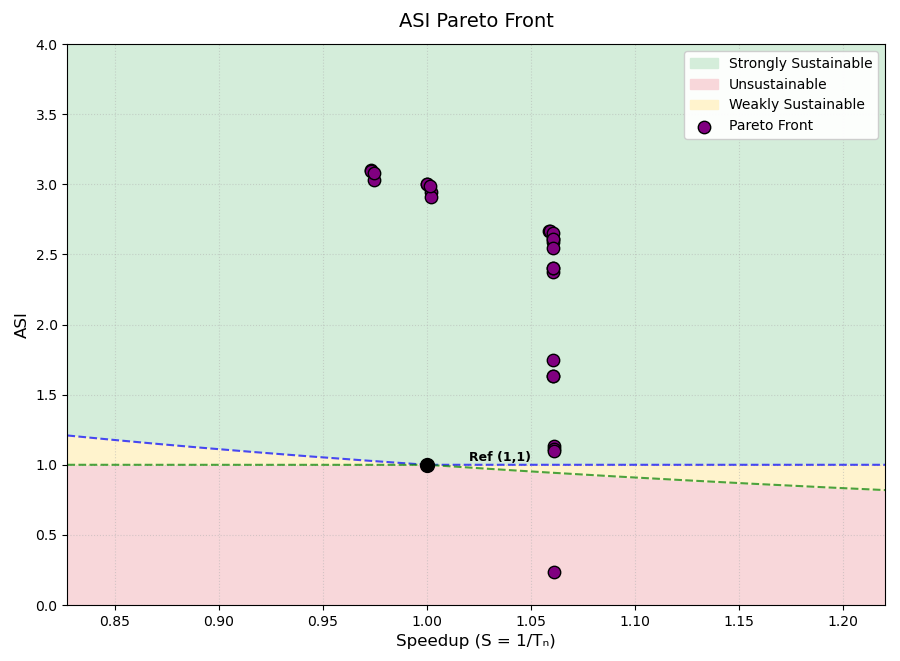
\includegraphics[width=0.48\textwidth]{../../images_results/ML2_greedy.png}
\end{figure}

\textbf{Result:}
\newline
Total sniper runs: 781
\newline
Final hypervolume: 3.2594

\textbf{Front:}

\begin{table}[H]
\centering
\resizebox{\textwidth}{!}{%
\begin{tabular}{lllllllllllllllllll}
\toprule
bpt & bp & l1da & l1d & l1ia & l1i & l2a & l2 & l3a & l3 & nhist & robc & robd & robw & ASI & Speedup & Area & PeakPow & Region \\
\midrule
a53 &  & 4 & 64 &  &  &  & 512 &  & 2048 & 4 &  &  & 1024 & 0.2323 & 1.0610 & 67.94 & 141.87 & Unsustainable \\
pentium\_m &  & 4 & 64 & 8 & 16 &  & 512 &  & 1024 &  & 8 & 2 & 1024 & 1.1008 & 1.0610 & 49.33 & 34.59 & Strongly Sust. \\
pentium\_m &  & 4 & 64 & 8 &  &  & 512 & 4 & 1024 &  & 2 & 2 & 1024 & 1.1154 & 1.0609 & 47.61 & 34.56 & Strongly Sust. \\
pentium\_m &  & 4 & 64 &  &  &  & 512 &  & 1024 &  &  & 2 & 1024 & 1.1342 & 1.0608 & 47.96 & 33.90 & Strongly Sust. \\
a53 &  &  & 64 &  &  &  & 512 &  & 2048 &  & 2 &  &  & 1.6355 & 1.0608 & 55.79 & 22.20 & Strongly Sust. \\
a53 & 512 &  & 64 &  &  &  & 512 &  & 2048 &  & 2 &  &  & 1.6355 & 1.0608 & 55.79 & 22.20 & Strongly Sust. \\
a53 &  &  & 64 &  &  &  & 512 &  & 2048 &  &  &  & 16 & 1.7450 & 1.0607 & 55.19 & 20.90 & Strongly Sust. \\
a53 & 512 &  & 64 &  &  &  & 512 &  & 1024 &  &  & 2 &  & 2.3749 & 1.0607 & 47.80 & 16.21 & Strongly Sust. \\
pentium\_m &  & 4 & 64 & 8 &  &  & 512 &  & 1024 &  &  & 2 & 64 & 2.4038 & 1.0607 & 45.04 & 16.33 & Strongly Sust. \\
a53 & 512 & 4 & 64 & 8 &  &  & 512 &  & 1024 &  &  & 2 & 64 & 2.4038 & 1.0606 & 45.04 & 16.33 & Strongly Sust. \\
a53 & 512 & 4 & 64 &  &  &  & 512 &  & 1024 &  &  & 2 & 64 & 2.5447 & 1.0606 & 43.32 & 15.61 & Strongly Sust. \\
a53 &  & 4 & 64 &  &  &  & 512 & 8 & 1024 &  &  & 2 & 64 & 2.5897 & 1.0606 & 41.24 & 15.56 & Strongly Sust. \\
a53 & 512 & 4 & 64 &  &  &  & 512 &  & 1024 &  &  & 2 & 16 & 2.6083 & 1.0606 & 43.17 & 15.25 & Strongly Sust. \\
a53 &  & 4 & 64 &  &  &  & 512 &  & 1024 &  &  & 2 & 16 & 2.6083 & 1.0605 & 43.17 & 15.25 & Strongly Sust. \\
a53 &  & 4 & 64 &  &  &  & 512 & 8 & 1024 &  &  & 2 & 16 & 2.6546 & 1.0605 & 41.09 & 15.19 & Strongly Sust. \\
a53 &  & 4 &  &  &  &  & 512 & 8 & 1024 &  &  & 2 & 16 & 2.6666 & 1.0589 & 40.92 & 15.14 & Strongly Sust. \\
a53 &  & 4 &  &  &  &  & 512 & 4 & 1024 &  &  & 2 & 16 & 2.6682 & 1.0589 & 40.92 & 15.13 & Strongly Sust. \\
a53 &  & 4 & 64 &  &  & 4 &  &  & 1024 &  &  & 2 & 32 & 2.9076 & 1.0019 & 36.49 & 14.31 & Strongly Sust. \\
a53 &  & 4 & 64 &  &  & 4 &  &  & 1024 &  &  & 2 & 16 & 2.9477 & 1.0018 & 36.40 & 14.12 & Strongly Sust. \\
a53 &  & 4 & 64 &  &  &  &  & 8 & 1024 &  &  & 2 & 16 & 2.9861 & 1.0013 & 34.86 & 14.08 & Strongly Sust. \\
a53 &  & 4 &  &  &  &  &  & 8 & 1024 &  &  & 2 & 16 & 3.0002 & 0.9999 & 34.69 & 14.03 & Strongly Sust. \\
a53 &  & 4 &  &  &  &  &  & 4 & 1024 &  &  & 2 & 16 & 3.0022 & 0.9999 & 34.69 & 14.02 & Strongly Sust. \\
a53 &  & 4 & 64 &  &  & 4 & 128 &  & 1024 &  &  & 2 & 16 & 3.0325 & 0.9746 & 35.43 & 13.81 & Strongly Sust. \\
a53 &  & 4 & 64 &  &  &  & 128 & 8 & 1024 &  &  & 2 & 16 & 3.0823 & 0.9744 & 33.37 & 13.77 & Strongly Sust. \\
a53 &  & 4 &  &  &  &  & 128 & 8 & 1024 &  &  & 2 & 16 & 3.0970 & 0.9732 & 33.20 & 13.72 & Strongly Sust. \\
a53 &  & 4 &  &  &  &  & 128 & 4 & 1024 &  &  & 2 & 16 & 3.0991 & 0.9731 & 33.20 & 13.71 & Strongly Sust. \\
\bottomrule
\end{tabular}
}
\end{table}


\subsection{SPEA2 - COLE}

\subsubsection{hyperparameter settings 1}
Hyperparameter settings: Patience = 1 (amount of iterations to wait before stopping after no improvement), max\_iterations: int = 10. (max iter never reached)

\begin{figure}[H]
\centering
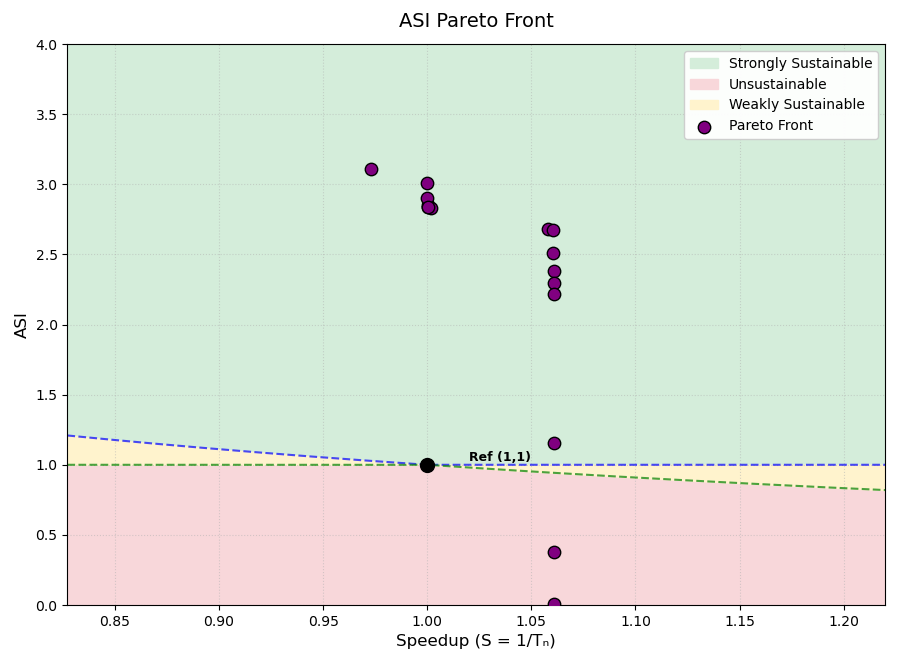
\includegraphics[width=0.48\textwidth]{../../images_results/ML2_spea2.png}
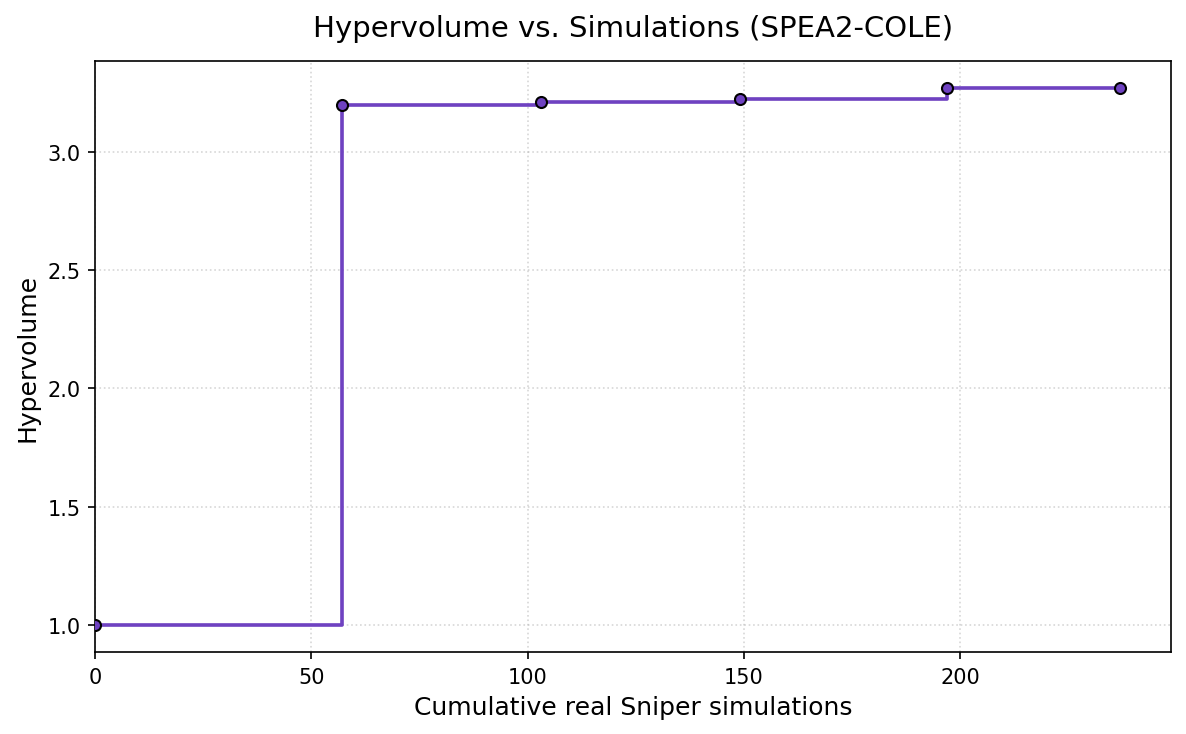
\includegraphics[width=0.48\textwidth]{../../images_results/ML2_spea2_hv_vs_sims.png}
\end{figure}

\textbf{Result:}
\newline
Total sniper runs: 237
\newline
Final hypervolume: 3.2693

\textbf{Front:}

\begin{table}[H]
\centering
\resizebox{\textwidth}{!}{%
\begin{tabular}{lllllllllllllllllll}
\toprule
bpt & bp & l1da & l1d & l1ia & l1i & l2a & l2 & l3a & l3 & nhist & robc & robd & robw & ASI & Speedup & Area & PeakPow & Region \\
\midrule
a53 & 1024 & 4 & 64 & 8 & 16 & 8 & 512 & 16 & 1024 & 3 & 2 & 8 & 1024 & 0.0070 & 1.0608 & 157.56 & 1188.00 & Unsustainable \\
pentium\_m &  & 8 & 64 & 4 & 16 & 8 & 512 & 16 & 1024 &  & 2 & 4 & 512 & 0.3748 & 1.0608 & 57.72 & 95.43 & Unsustainable \\
pentium\_m &  & 4 & 64 & 4 & 16 & 8 & 512 & 4 & 1024 &  & 2 & 2 & 1024 & 1.1558 & 1.0608 & 45.64 & 33.82 & Strongly Sust. \\
pentium\_m &  & 4 & 64 & 8 & 64 & 4 & 512 & 8 & 2048 &  & 4 & 2 & 256 & 2.2207 & 1.0607 & 48.56 & 17.24 & Strongly Sust. \\
tage &  & 4 & 64 & 8 & 16 & 8 & 512 & 4 & 2048 &  & 10 & 2 & 16 & 2.2940 & 1.0607 & 49.42 & 16.59 & Strongly Sust. \\
pentium\_m &  & 4 & 64 & 4 & 32 & 8 & 512 & 16 & 2048 &  & 4 & 2 & 32 & 2.3800 & 1.0606 & 48.12 & 16.14 & Strongly Sust. \\
pentium\_m &  & 4 & 64 & 8 & 64 & 8 & 512 & 4 & 1024 &  & 10 & 2 & 16 & 2.5075 & 1.0605 & 43.13 & 15.86 & Strongly Sust. \\
tage &  & 4 & 64 & 4 & 16 & 4 & 512 & 4 & 1024 &  & 8 & 2 & 16 & 2.6748 & 1.0605 & 40.76 & 15.11 & Strongly Sust. \\
tage &  & 4 & 16 & 4 & 32 & 8 & 512 & 4 & 1024 &  & 4 & 2 & 16 & 2.6778 & 1.0581 & 40.73 & 15.10 & Strongly Sust. \\
pentium\_m &  & 4 & 64 & 8 & 64 & 4 & 256 & 8 & 1024 &  & 2 & 2 & 16 & 2.8286 & 1.0018 & 36.35 & 14.72 & Strongly Sust. \\
pentium\_m &  & 4 & 32 & 8 & 64 & 4 & 256 & 8 & 1024 &  & 10 & 2 & 16 & 2.8417 & 1.0004 & 36.18 & 14.67 & Strongly Sust. \\
pentium\_m &  & 4 & 32 & 8 & 64 & 4 & 256 & 8 & 1024 &  & 10 & 2 & 16 & 2.8417 & 1.0004 & 36.18 & 14.67 & Strongly Sust. \\
pentium\_m &  & 4 & 32 & 8 & 16 & 4 & 256 & 4 & 1024 &  & 10 & 2 & 16 & 2.8550 & 1.0003 & 35.52 & 14.66 & Strongly Sust. \\
pentium\_m &  & 4 & 32 & 4 & 16 & 8 & 256 & 4 & 1024 &  & 10 & 2 & 128 & 2.9034 & 1.0000 & 34.66 & 14.50 & Strongly Sust. \\
pentium\_m &  & 4 & 32 & 4 & 16 & 8 & 256 & 4 & 1024 &  & 2 & 2 & 16 & 3.0118 & 0.9999 & 34.45 & 14.00 & Strongly Sust. \\
pentium\_m &  & 4 & 32 & 4 & 16 & 8 & 128 & 4 & 1024 &  & 2 & 2 & 16 & 3.1091 & 0.9731 & 32.96 & 13.69 & Strongly Sust. \\
\bottomrule
\end{tabular}
}
\end{table}


\subsection{Max-value Entropy Search for Multi-objective Bayesian Optimization (MESMO)}
source: \url{https://arxiv.org/pdf/2110.06980}
\subsubsection{hyperparameter settings 1}
Hyperparameter settings: 400 candidate samples (400 candidate configurations are considered per iteration; each is scored by the information gained, averaged over a default of 10 Monte Carlo posterior-function samples (amount is hyperparameter, default is 10), and the top-scoring one (also hyperparameter, default is 1) is evaluated.) are used and 7 initial configurations (including baseline, always the case!) have been run.

\begin{itemize}

\item 20 iterations
\begin{figure}[H]
\centering
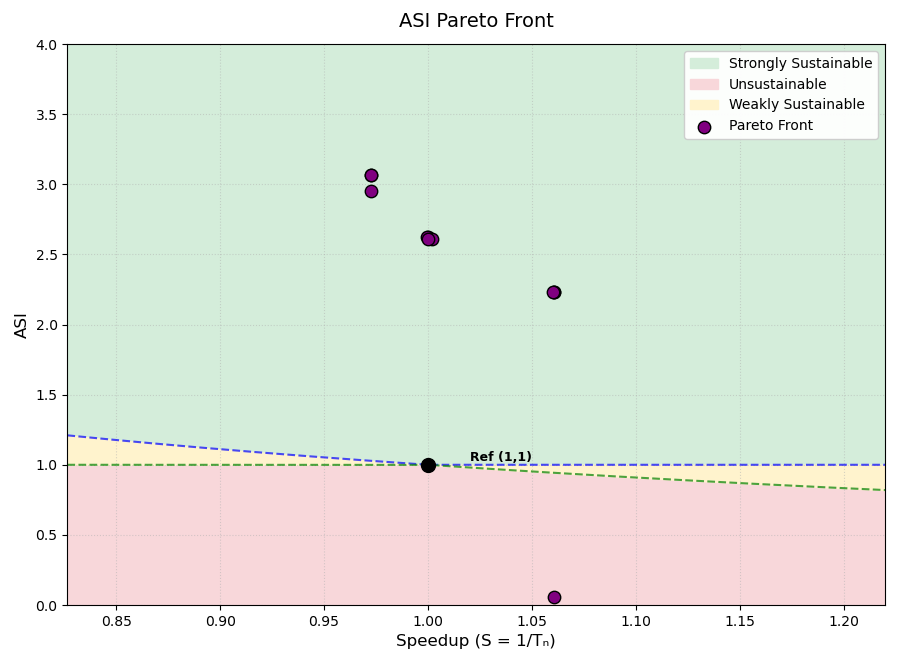
\includegraphics[width=0.48\textwidth]{../../images_results/ML2_mesmo_400_20iters.png}
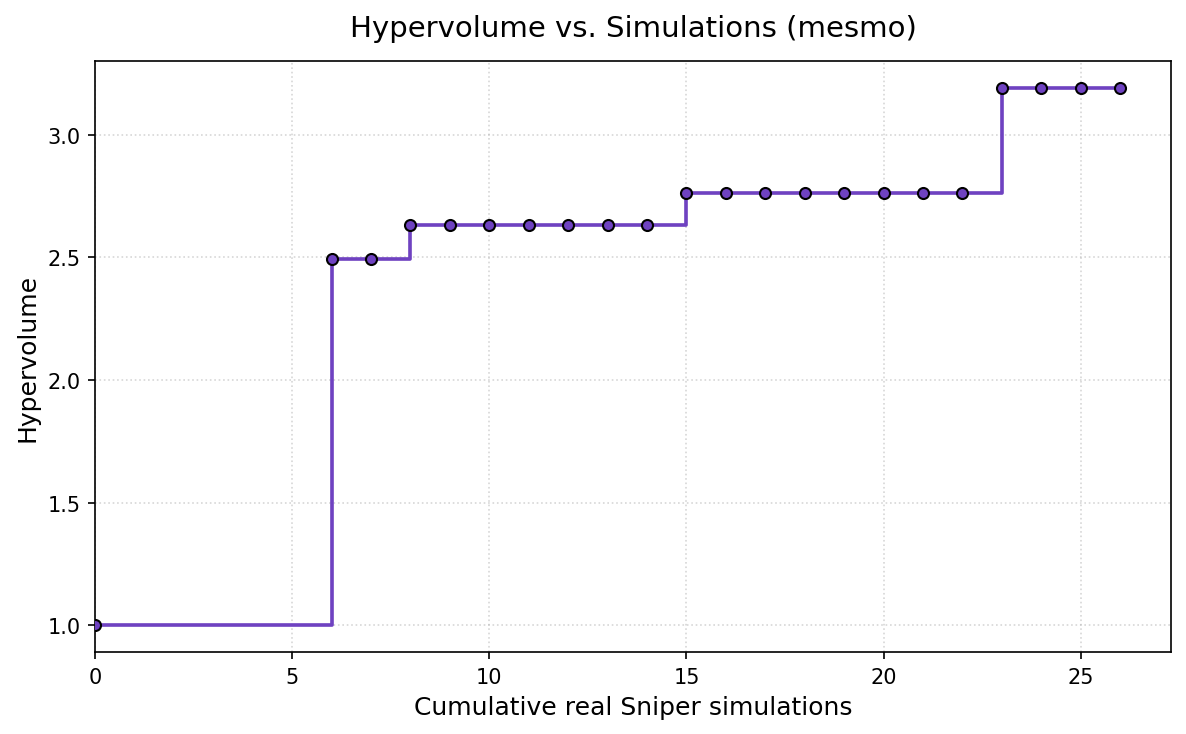
\includegraphics[width=0.48\textwidth]{../../images_results/ML2_mesmo_400_20iters_hv_vs_sims.png}
\end{figure}

\textbf{Result:}
\newline
Total sniper runs: 26
\newline
Final hypervolume: 3.1908

\textbf{Front:}

\begin{table}[H]
\centering
\resizebox{\textwidth}{!}{%
\begin{tabular}{lllllllllllllllllllll}
\toprule
bpt & bp & l1da & l1d & l1ia & l1i & l2a & l2 & l3a & l3 & nhist & nnbl & nnlr & robc & robd & robw & ASI & Speedup & Area & PeakPow & Region \\
\midrule
pentium\_m &  & 8 & 64 & 8 & 16 & 8 & 512 & 16 & 1024 &  &  &  & 10 & 8 & 256 & 0.0537 & 1.0608 & 83.61 & 533.35 & Unsustainable \\
a53 & 512 & 8 & 64 & 8 & 16 & 8 & 512 & 16 & 1024 & 2 &  &  & 10 & 2 & 256 & 2.2291 & 1.0606 & 49.29 & 17.09 & Strongly Sust. \\
pentium\_m &  & 8 & 64 & 8 & 16 & 8 & 512 & 16 & 1024 &  &  &  & 10 & 2 & 256 & 2.2292 & 1.0605 & 49.29 & 17.08 & Strongly Sust. \\
nn &  & 8 & 64 & 8 & 16 & 8 & 512 & 16 & 1024 &  & 16 & 0.005 & 10 & 2 & 256 & 2.2293 & 1.0602 & 49.29 & 17.08 & Strongly Sust. \\
a53 & 512 & 4 & 64 & 4 & 16 & 4 & 256 & 4 & 2048 & 4 &  &  & 2 & 2 & 256 & 2.6064 & 1.0018 & 41.36 & 15.45 & Strongly Sust. \\
nn &  & 4 & 64 & 4 & 16 & 4 & 256 & 4 & 2048 &  & 16 & 0.0005 & 2 & 2 & 256 & 2.6071 & 1.0001 & 41.36 & 15.44 & Strongly Sust. \\
pentium\_m &  & 4 & 16 & 4 & 16 & 4 & 256 & 4 & 2048 &  &  &  & 2 & 2 & 256 & 2.6273 & 0.9999 & 40.99 & 15.36 & Strongly Sust. \\
a53 & 512 & 4 & 16 & 4 & 16 & 4 & 256 & 4 & 2048 & 4 &  &  & 2 & 2 & 256 & 2.6273 & 0.9997 & 40.99 & 15.36 & Strongly Sust. \\
a53 & 512 & 4 & 16 & 4 & 32 & 8 & 128 & 4 & 1024 & 4 &  &  & 2 & 2 & 256 & 2.9545 & 0.9724 & 33.33 & 14.37 & Strongly Sust. \\
a53 & 512 & 4 & 16 & 4 & 32 & 8 & 128 & 4 & 1024 & 4 &  &  & 4 & 2 & 32 & 3.0672 & 0.9723 & 33.09 & 13.87 & Strongly Sust. \\
a53 & 512 & 4 & 16 & 4 & 32 & 8 & 128 & 4 & 1024 & 4 &  &  & 2 & 2 & 32 & 3.0672 & 0.9723 & 33.09 & 13.87 & Strongly Sust. \\
\bottomrule
\end{tabular}
}
\end{table}

\item 60 iterations
\begin{figure}[H]
\centering
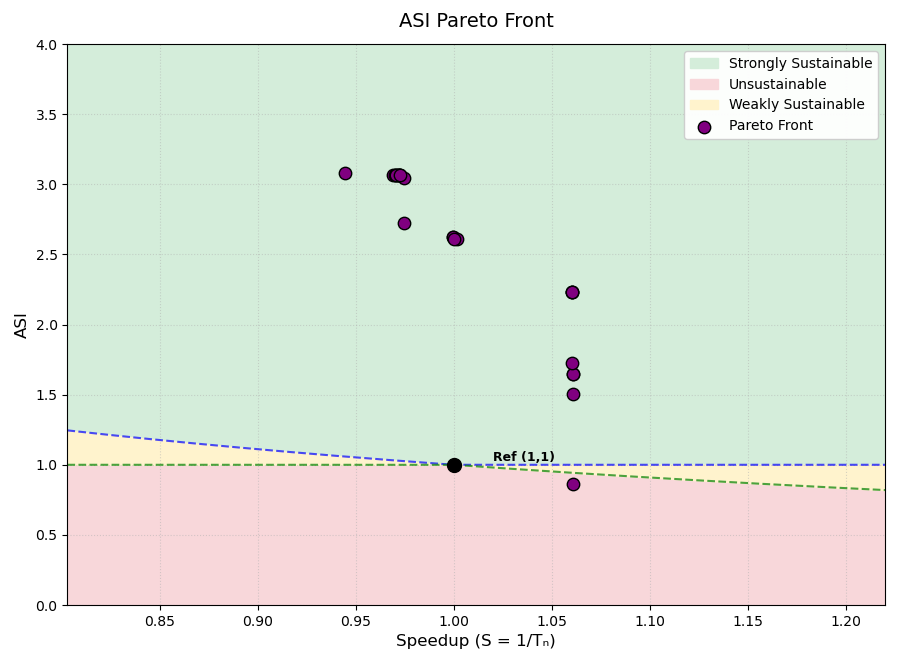
\includegraphics[width=0.48\textwidth]{../../images_results/ML2_mesmo_400_60iters.png}
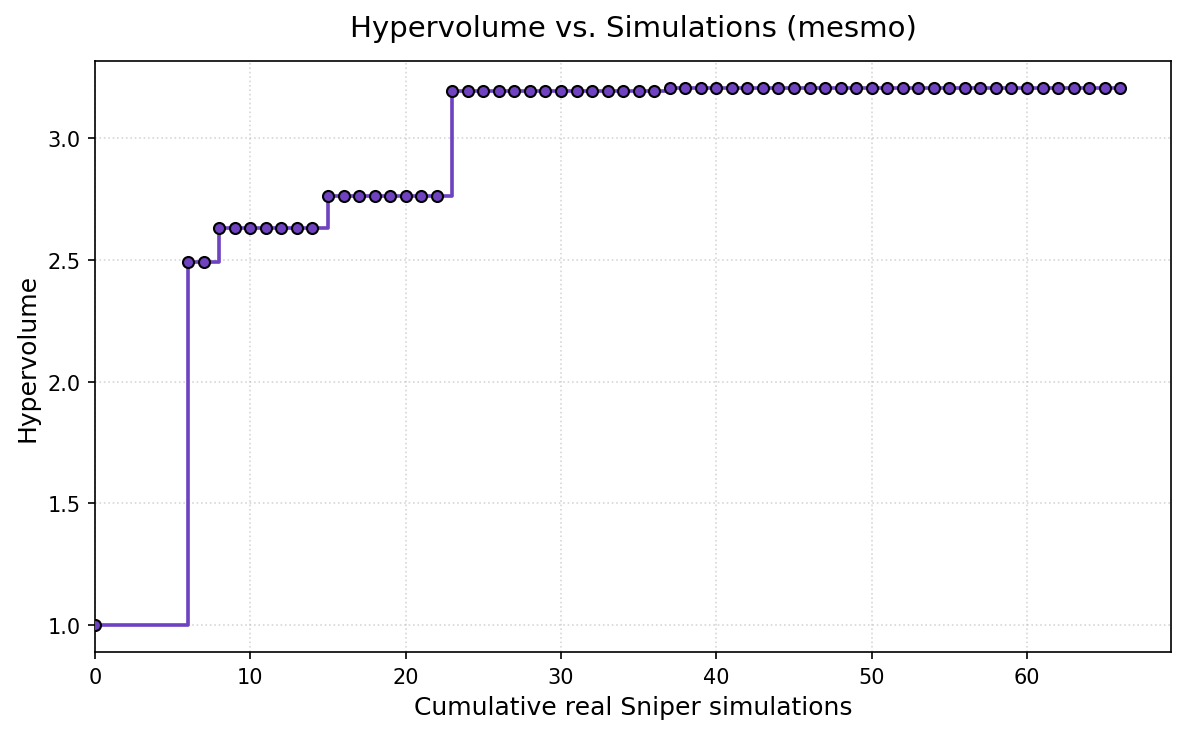
\includegraphics[width=0.48\textwidth]{../../images_results/ML2_mesmo_400_60iters_hv_vs_sims.png}
\end{figure}

\textbf{Result:}
\newline
Total sniper runs: 66
\newline
Final hypervolume: 3.2056

\textbf{Front:}

\begin{table}[H]
\centering
\resizebox{\textwidth}{!}{%
\begin{tabular}{lllllllllllllllllllll}
\toprule
bpt & bp & l1da & l1d & l1ia & l1i & l2a & l2 & l3a & l3 & nhist & nnbl & nnlr & robc & robd & robw & ASI & Speedup & Area & PeakPow & Region \\
\midrule
pentium\_m &  & 8 & 64 & 8 & 16 & 4 & 512 & 8 & 4096 &  &  &  & 10 & 2 & 1024 & 0.8626 & 1.0609 & 70.94 & 37.26 & Unsustainable \\
pentium\_m &  & 8 & 64 & 8 & 16 & 8 & 512 & 16 & 1024 &  &  &  & 10 & 2 & 512 & 1.5034 & 1.0608 & 50.78 & 25.06 & Strongly Sust. \\
pentium\_m &  & 4 & 64 & 8 & 64 & 8 & 512 & 16 & 2048 &  &  &  & 10 & 4 & 128 & 1.6488 & 1.0608 & 53.40 & 22.41 & Strongly Sust. \\
pentium\_m &  & 4 & 64 & 8 & 64 & 8 & 512 & 16 & 2048 &  &  &  & 8 & 4 & 128 & 1.6488 & 1.0607 & 53.40 & 22.41 & Strongly Sust. \\
a53 & 512 & 8 & 64 & 8 & 16 & 8 & 512 & 16 & 4096 & 2 &  &  & 10 & 2 & 256 & 1.7280 & 1.0606 & 66.19 & 19.35 & Strongly Sust. \\
a53 & 512 & 8 & 64 & 8 & 16 & 8 & 512 & 16 & 1024 & 2 &  &  & 10 & 2 & 256 & 2.2291 & 1.0606 & 49.29 & 17.09 & Strongly Sust. \\
pentium\_m &  & 8 & 64 & 8 & 16 & 8 & 512 & 16 & 1024 &  &  &  & 10 & 2 & 256 & 2.2292 & 1.0605 & 49.29 & 17.08 & Strongly Sust. \\
nn &  & 8 & 64 & 8 & 16 & 8 & 512 & 16 & 1024 &  & 16 & 0.005 & 10 & 2 & 256 & 2.2293 & 1.0602 & 49.29 & 17.08 & Strongly Sust. \\
a53 & 512 & 4 & 64 & 4 & 16 & 4 & 256 & 4 & 2048 & 4 &  &  & 2 & 2 & 256 & 2.6064 & 1.0018 & 41.36 & 15.45 & Strongly Sust. \\
nn &  & 4 & 64 & 4 & 16 & 4 & 256 & 4 & 2048 &  & 16 & 0.0005 & 2 & 2 & 256 & 2.6071 & 1.0001 & 41.36 & 15.44 & Strongly Sust. \\
pentium\_m &  & 4 & 16 & 4 & 16 & 4 & 256 & 4 & 2048 &  &  &  & 2 & 2 & 256 & 2.6273 & 0.9999 & 40.99 & 15.36 & Strongly Sust. \\
a53 & 512 & 4 & 16 & 4 & 16 & 4 & 256 & 4 & 2048 & 4 &  &  & 2 & 2 & 256 & 2.6273 & 0.9997 & 40.99 & 15.36 & Strongly Sust. \\
tage &  & 4 & 64 & 4 & 32 & 4 & 128 & 16 & 2048 &  &  &  & 4 & 2 & 64 & 2.7216 & 0.9747 & 40.44 & 14.89 & Strongly Sust. \\
nn &  & 4 & 64 & 4 & 32 & 8 & 128 & 4 & 1024 &  & 64 & 0.0005 & 8 & 2 & 32 & 3.0414 & 0.9746 & 33.46 & 13.95 & Strongly Sust. \\
a53 & 512 & 4 & 16 & 4 & 32 & 8 & 128 & 4 & 1024 & 3 &  &  & 8 & 2 & 32 & 3.0671 & 0.9725 & 33.09 & 13.87 & Strongly Sust. \\
a53 & 512 & 4 & 16 & 4 & 32 & 8 & 128 & 4 & 1024 & 4 &  &  & 10 & 2 & 32 & 3.0671 & 0.9724 & 33.09 & 13.87 & Strongly Sust. \\
tage &  & 4 & 16 & 4 & 32 & 8 & 128 & 4 & 1024 &  &  &  & 2 & 2 & 32 & 3.0672 & 0.9723 & 33.09 & 13.87 & Strongly Sust. \\
a53 & 512 & 4 & 16 & 4 & 32 & 8 & 128 & 4 & 1024 & 4 &  &  & 8 & 2 & 32 & 3.0672 & 0.9723 & 33.09 & 13.87 & Strongly Sust. \\
nn &  & 4 & 16 & 4 & 32 & 8 & 128 & 4 & 1024 &  & 16 & 0.0005 & 10 & 2 & 32 & 3.0675 & 0.9717 & 33.09 & 13.87 & Strongly Sust. \\
nn &  & 4 & 16 & 4 & 32 & 8 & 128 & 4 & 1024 &  & 64 & 0.005 & 2 & 2 & 32 & 3.0681 & 0.9706 & 33.09 & 13.86 & Strongly Sust. \\
nn &  & 4 & 16 & 4 & 32 & 8 & 128 & 4 & 1024 &  & 64 & 0.005 & 10 & 2 & 32 & 3.0682 & 0.9703 & 33.09 & 13.86 & Strongly Sust. \\
nn &  & 4 & 16 & 4 & 32 & 8 & 128 & 4 & 1024 &  & 32 & 0.0005 & 10 & 2 & 32 & 3.0684 & 0.9700 & 33.09 & 13.86 & Strongly Sust. \\
nn &  & 4 & 16 & 4 & 32 & 8 & 128 & 4 & 1024 &  & 32 & 0.0005 & 8 & 2 & 32 & 3.0688 & 0.9692 & 33.09 & 13.86 & Strongly Sust. \\
nn &  & 4 & 16 & 4 & 32 & 8 & 128 & 4 & 1024 &  & 64 & 0.0005 & 8 & 2 & 32 & 3.0814 & 0.9447 & 33.09 & 13.80 & Strongly Sust. \\
\bottomrule
\end{tabular}
}
\end{table}


\item 200 iterations
\begin{figure}[H]
\centering
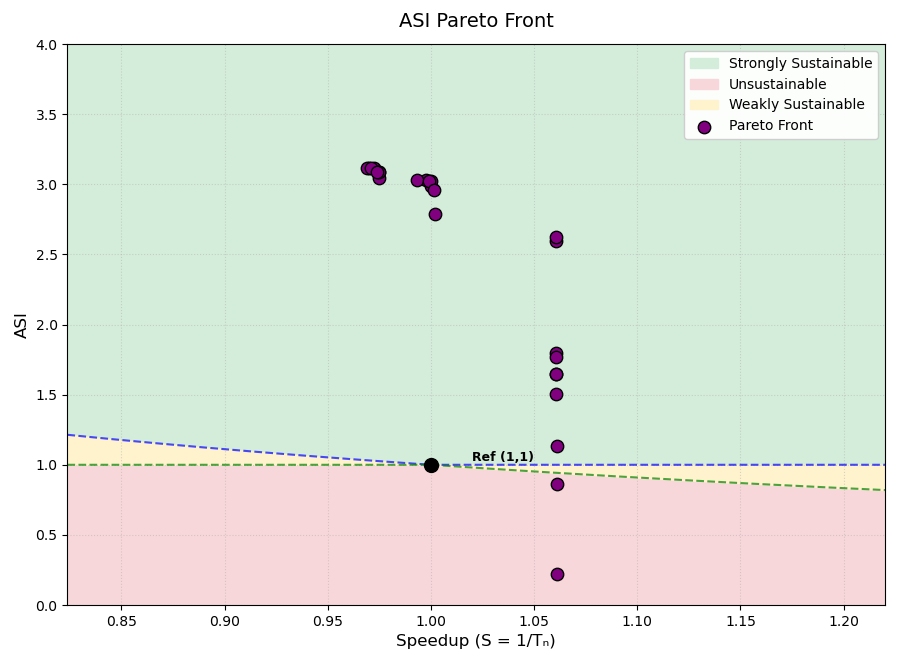
\includegraphics[width=0.48\textwidth]{../../images_results/ML2_mesmo_400_200iters.png}
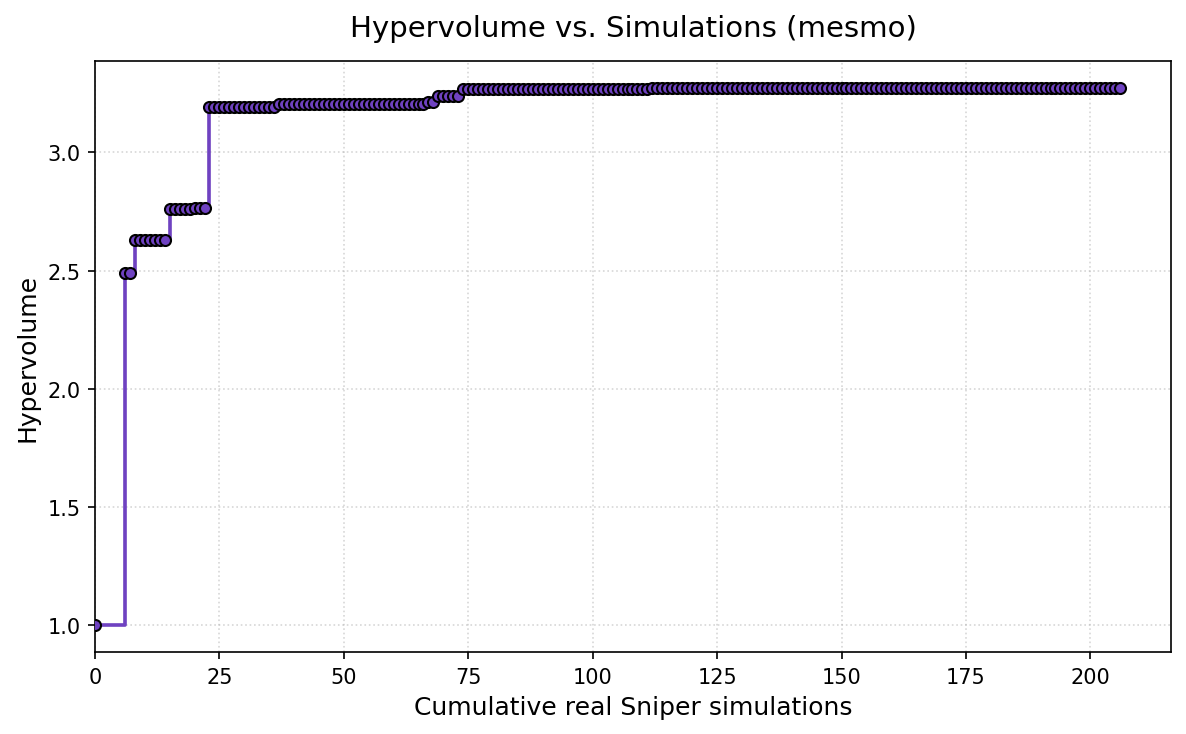
\includegraphics[width=0.48\textwidth]{../../images_results/ML2_mesmo_400_200iters_hv_vs_sims.png}
\end{figure}

\textbf{Result:}
\newline
Total sniper runs: 206
\newline
Final hypervolume: 3.2729

\textbf{Front:}

\begin{table}[H]
\centering
\resizebox{\textwidth}{!}{%
\begin{tabular}{lllllllllllllllllllll}
\toprule
bpt & bp & l1da & l1d & l1ia & l1i & l2a & l2 & l3a & l3 & nhist & nnbl & nnlr & robc & robd & robw & ASI & Speedup & Area & PeakPow & Region \\
\midrule
pentium\_m &  & 8 & 64 & 4 & 64 & 8 & 512 & 4 & 2048 &  &  &  & 8 & 4 & 1024 & 0.2219 & 1.0609 & 72.96 & 142.35 & Unsustainable \\
pentium\_m &  & 8 & 64 & 8 & 16 & 4 & 512 & 8 & 4096 &  &  &  & 10 & 2 & 1024 & 0.8626 & 1.0609 & 70.94 & 37.26 & Unsustainable \\
pentium\_m &  & 4 & 64 & 4 & 16 & 8 & 512 & 16 & 1024 &  &  &  & 2 & 2 & 1024 & 1.1369 & 1.0609 & 47.72 & 33.88 & Strongly Sust. \\
pentium\_m &  & 8 & 64 & 8 & 16 & 8 & 512 & 16 & 1024 &  &  &  & 10 & 2 & 512 & 1.5034 & 1.0608 & 50.78 & 25.06 & Strongly Sust. \\
pentium\_m &  & 4 & 64 & 8 & 64 & 8 & 512 & 16 & 2048 &  &  &  & 10 & 4 & 128 & 1.6488 & 1.0608 & 53.40 & 22.41 & Strongly Sust. \\
pentium\_m &  & 4 & 64 & 8 & 64 & 8 & 512 & 16 & 2048 &  &  &  & 8 & 4 & 128 & 1.6488 & 1.0607 & 53.40 & 22.41 & Strongly Sust. \\
pentium\_m &  & 8 & 64 & 8 & 64 & 8 & 512 & 16 & 4096 &  &  &  & 8 & 2 & 32 & 1.7692 & 1.0606 & 66.61 & 18.84 & Strongly Sust. \\
pentium\_m &  & 4 & 64 & 8 & 32 & 8 & 512 & 16 & 1024 &  &  &  & 8 & 4 & 64 & 1.7965 & 1.0606 & 48.05 & 21.39 & Strongly Sust. \\
pentium\_m &  & 4 & 64 & 4 & 16 & 8 & 512 & 8 & 1024 &  &  &  & 10 & 2 & 64 & 2.5978 & 1.0606 & 41.00 & 15.54 & Strongly Sust. \\
nn &  & 4 & 64 & 4 & 32 & 8 & 512 & 4 & 1024 &  & 64 & 0.0005 & 8 & 2 & 32 & 2.6225 & 1.0606 & 41.18 & 15.37 & Strongly Sust. \\
tage &  & 8 & 64 & 4 & 32 & 4 & 256 & 8 & 1024 &  &  &  & 2 & 2 & 32 & 2.7856 & 1.0019 & 38.83 & 14.70 & Strongly Sust. \\
a53 & 2048 & 4 & 64 & 4 & 64 & 8 & 256 & 8 & 1024 & 2 &  &  & 4 & 2 & 16 & 2.9603 & 1.0013 & 35.45 & 14.15 & Strongly Sust. \\
nn &  & 4 & 32 & 4 & 64 & 4 & 256 & 4 & 1024 &  & 16 & 0.005 & 2 & 2 & 16 & 2.9891 & 1.0002 & 34.74 & 14.08 & Strongly Sust. \\
nn &  & 4 & 32 & 4 & 16 & 4 & 256 & 4 & 1024 &  & 16 & 0.005 & 10 & 2 & 16 & 3.0249 & 1.0002 & 33.91 & 13.99 & Strongly Sust. \\
nn &  & 4 & 16 & 4 & 32 & 4 & 256 & 4 & 1024 &  & 16 & 0.005 & 10 & 2 & 16 & 3.0264 & 0.9993 & 33.96 & 13.97 & Strongly Sust. \\
nn &  & 4 & 16 & 4 & 32 & 4 & 256 & 4 & 1024 &  & 64 & 0.005 & 10 & 2 & 16 & 3.0272 & 0.9977 & 33.96 & 13.97 & Strongly Sust. \\
nn &  & 4 & 32 & 4 & 16 & 4 & 256 & 4 & 1024 &  & 16 & 0.0005 & 10 & 2 & 16 & 3.0284 & 0.9932 & 33.91 & 13.97 & Strongly Sust. \\
a53 & 2048 & 4 & 64 & 4 & 32 & 4 & 128 & 4 & 1024 & 4 &  &  & 8 & 2 & 32 & 3.0444 & 0.9746 & 33.43 & 13.94 & Strongly Sust. \\
a53 & 2048 & 4 & 64 & 4 & 32 & 4 & 128 & 4 & 1024 & 4 &  &  & 8 & 2 & 16 & 3.0873 & 0.9746 & 33.35 & 13.75 & Strongly Sust. \\
a53 & 512 & 4 & 64 & 4 & 32 & 4 & 128 & 4 & 1024 & 4 &  &  & 8 & 2 & 16 & 3.0873 & 0.9746 & 33.35 & 13.75 & Strongly Sust. \\
nn &  & 4 & 64 & 4 & 32 & 4 & 128 & 4 & 1024 &  & 16 & 0.0005 & 8 & 2 & 16 & 3.0877 & 0.9738 & 33.35 & 13.75 & Strongly Sust. \\
tage &  & 4 & 16 & 4 & 32 & 4 & 128 & 4 & 1024 &  &  &  & 10 & 2 & 16 & 3.1136 & 0.9724 & 32.98 & 13.67 & Strongly Sust. \\
nn &  & 4 & 16 & 4 & 32 & 4 & 128 & 4 & 1024 &  & 16 & 0.001 & 10 & 2 & 16 & 3.1144 & 0.9709 & 32.98 & 13.67 & Strongly Sust. \\
nn &  & 4 & 16 & 4 & 32 & 4 & 128 & 4 & 1024 &  & 64 & 0.005 & 10 & 2 & 16 & 3.1149 & 0.9699 & 32.98 & 13.66 & Strongly Sust. \\
nn &  & 4 & 16 & 4 & 32 & 4 & 128 & 4 & 1024 &  & 64 & 0.001 & 10 & 2 & 16 & 3.1153 & 0.9692 & 32.98 & 13.66 & Strongly Sust. \\
\bottomrule
\end{tabular}
}
\end{table}
\end{itemize}

HV was already 3.2727 at iter 152, before that also quite slow increase. Amount of points did increase with 10.
\section{ML2 and CCl benchmarks}
ML2: L2 resident (depending on LFSR settings) linked list traversal
\newline
CCl: Impossible control with large basic blocks (potentially larger penalty)
\subsection{Greedy}

Became infeasable with new parameterspace. \\
first iteration: 33 simulations \\
second iteration: \(\ge\)100 simulations
\subsection{SPEA2 - COLE}

\subsubsection{hyperparameter settings 1}

Hyperparameter settings: Patience = 1 (amount of iterations to wait before stopping after no improvement), max\_iterations: int = 30, \\
folowing parameters are default: num\_populations: int = 3, population\_size: int = 20, archive\_size: int = 10, p\_mutation: float = 0.10, p\_crossover: float = 0.90, p\_migration: float = 0.10.

\begin{figure}[H]
\centering
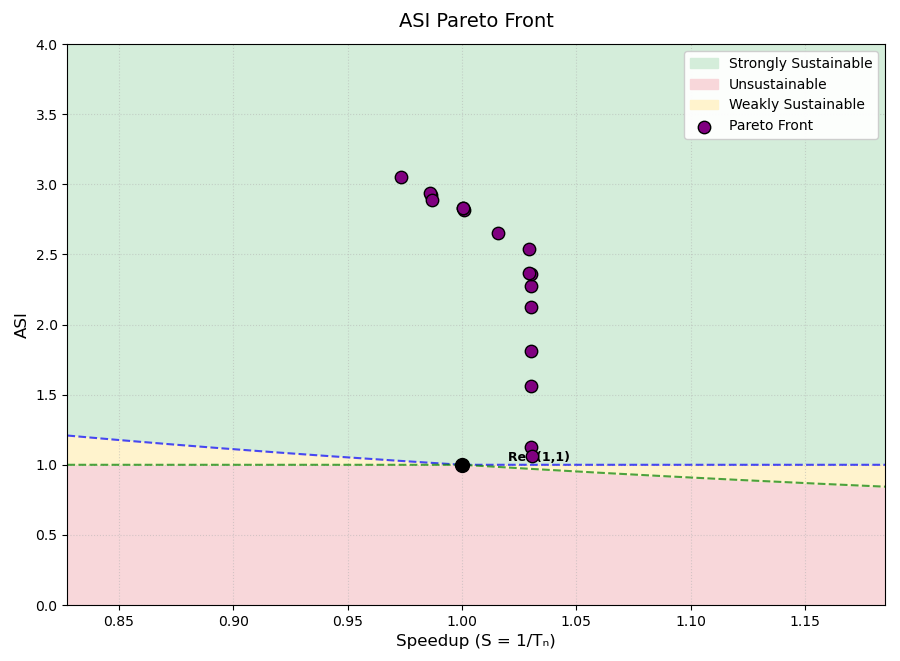
\includegraphics[width=0.48\textwidth]{../../images_results/ML2_and_CCl_spea2.png}
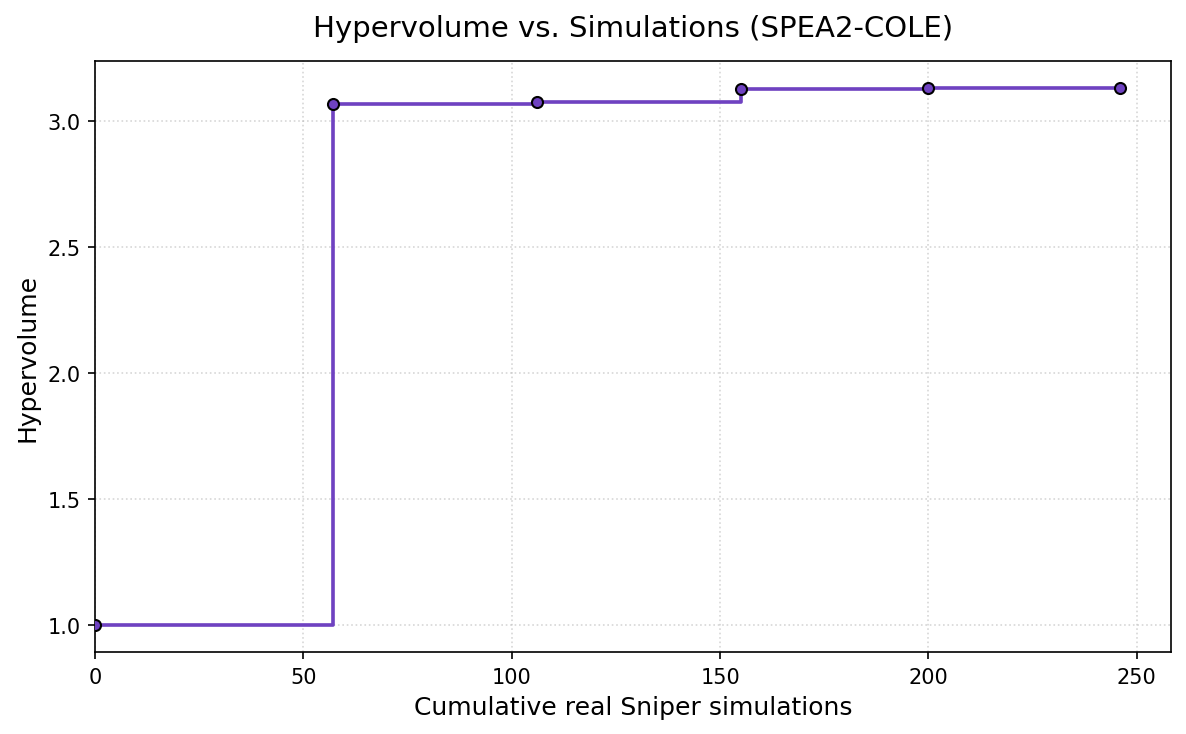
\includegraphics[width=0.48\textwidth]{../../images_results/ML2_and_CCl_spea2_hv_vs_sims.png}
\end{figure}

\textbf{Result:}
\newline
Total sniper runs: 246
\newline
Final hypervolume: 3.1294

\textbf{Front:}

\begin{table}[H]
\centering
\resizebox{\textwidth}{!}{%
\begin{tabular}{lllllllllllllllllllll}
\toprule
bpt & bp & l1da & l1d & l1ia & l1i & l2a & l2 & l3a & l3 & nhist & nnbl & nnlr & robc & robd & robw & ASI & Speedup & Area & PeakPow & Region \\
\midrule
a53 & 1024 & 4 & 64 & 8 & 64 & 8 & 512 & 8 & 2048 & 3 &  &  & 4 & 2 & 1024 & 1.0624 & 1.0304 & 53.11 & 36.02 & Strongly Sust. \\
a53 & 1024 & 4 & 64 & 8 & 64 & 4 & 512 & 8 & 1024 & 3 &  &  & 4 & 2 & 1024 & 1.1281 & 1.0303 & 47.82 & 35.26 & Strongly Sust. \\
pentium\_m &  & 4 & 64 & 4 & 16 & 4 & 512 & 4 & 2048 &  &  &  & 2 & 2 & 512 & 1.5617 & 1.0302 & 49.53 & 25.16 & Strongly Sust. \\
pentium\_m &  & 4 & 64 & 8 & 64 & 8 & 512 & 16 & 4096 &  &  &  & 10 & 2 & 256 & 1.8130 & 1.0302 & 62.43 & 19.65 & Strongly Sust. \\
pentium\_m &  & 8 & 64 & 4 & 64 & 8 & 512 & 16 & 2048 &  &  &  & 4 & 2 & 256 & 2.1272 & 1.0302 & 53.37 & 17.96 & Strongly Sust. \\
pentium\_m &  & 4 & 64 & 4 & 64 & 8 & 512 & 4 & 2048 &  &  &  & 2 & 2 & 256 & 2.2773 & 1.0302 & 48.96 & 17.32 & Strongly Sust. \\
pentium\_m &  & 8 & 64 & 4 & 32 & 4 & 512 & 4 & 1024 &  &  &  & 2 & 2 & 256 & 2.3633 & 1.0301 & 45.75 & 17.08 & Strongly Sust. \\
pentium\_m &  & 8 & 32 & 4 & 32 & 8 & 512 & 4 & 1024 &  &  &  & 4 & 2 & 256 & 2.3675 & 1.0293 & 45.51 & 17.08 & Strongly Sust. \\
pentium\_m &  & 4 & 32 & 4 & 16 & 4 & 512 & 4 & 1024 &  &  &  & 2 & 2 & 256 & 2.5419 & 1.0293 & 40.92 & 16.42 & Strongly Sust. \\
pentium\_m &  & 4 & 32 & 4 & 32 & 8 & 512 & 8 & 1024 &  &  &  & 4 & 2 & 16 & 2.6494 & 1.0158 & 40.92 & 15.75 & Strongly Sust. \\
a53 & 512 & 4 & 64 & 4 & 16 & 4 & 256 & 4 & 1024 & 2 &  &  & 4 & 2 & 256 & 2.8179 & 1.0009 & 34.41 & 15.47 & Strongly Sust. \\
pentium\_m &  & 4 & 32 & 4 & 16 & 4 & 256 & 4 & 1024 &  &  &  & 4 & 2 & 256 & 2.8307 & 1.0005 & 34.23 & 15.41 & Strongly Sust. \\
pentium\_m &  & 4 & 32 & 4 & 16 & 4 & 256 & 4 & 1024 &  &  &  & 4 & 2 & 256 & 2.8307 & 1.0005 & 34.23 & 15.41 & Strongly Sust. \\
pentium\_m &  & 4 & 32 & 4 & 32 & 8 & 128 & 8 & 1024 &  &  &  & 4 & 2 & 256 & 2.8878 & 0.9868 & 33.52 & 15.18 & Strongly Sust. \\
a53 & 512 & 4 & 32 & 4 & 32 & 8 & 128 & 8 & 1024 & 3 &  &  & 4 & 2 & 128 & 2.9270 & 0.9865 & 33.40 & 14.99 & Strongly Sust. \\
a53 & 1024 & 4 & 16 & 4 & 32 & 8 & 128 & 8 & 1024 & 3 &  &  & 4 & 2 & 128 & 2.9384 & 0.9861 & 33.21 & 14.95 & Strongly Sust. \\
pentium\_m &  & 4 & 16 & 4 & 32 & 8 & 128 & 8 & 1024 &  &  &  & 4 & 2 & 16 & 3.0553 & 0.9734 & 33.00 & 14.39 & Strongly Sust. \\
\bottomrule
\end{tabular}
}
\end{table}


\subsection{MESMO}

\subsubsection{hyperparameter settings 1}
hyperparameter settings: 200 candidate samples (200 candidate configurations are considered per iteration; each is scored by the information gained, averaged over a default of 10 Monte Carlo posterior-function samples (amount is hyperparameter, default is 10), and the top-scoring one (also hyperparameter, default is 1) is evaluated.) are used and 5 initial configurations (including baseline, always the case!) have been run. 20 iterations.

\begin{figure}[H]
\centering
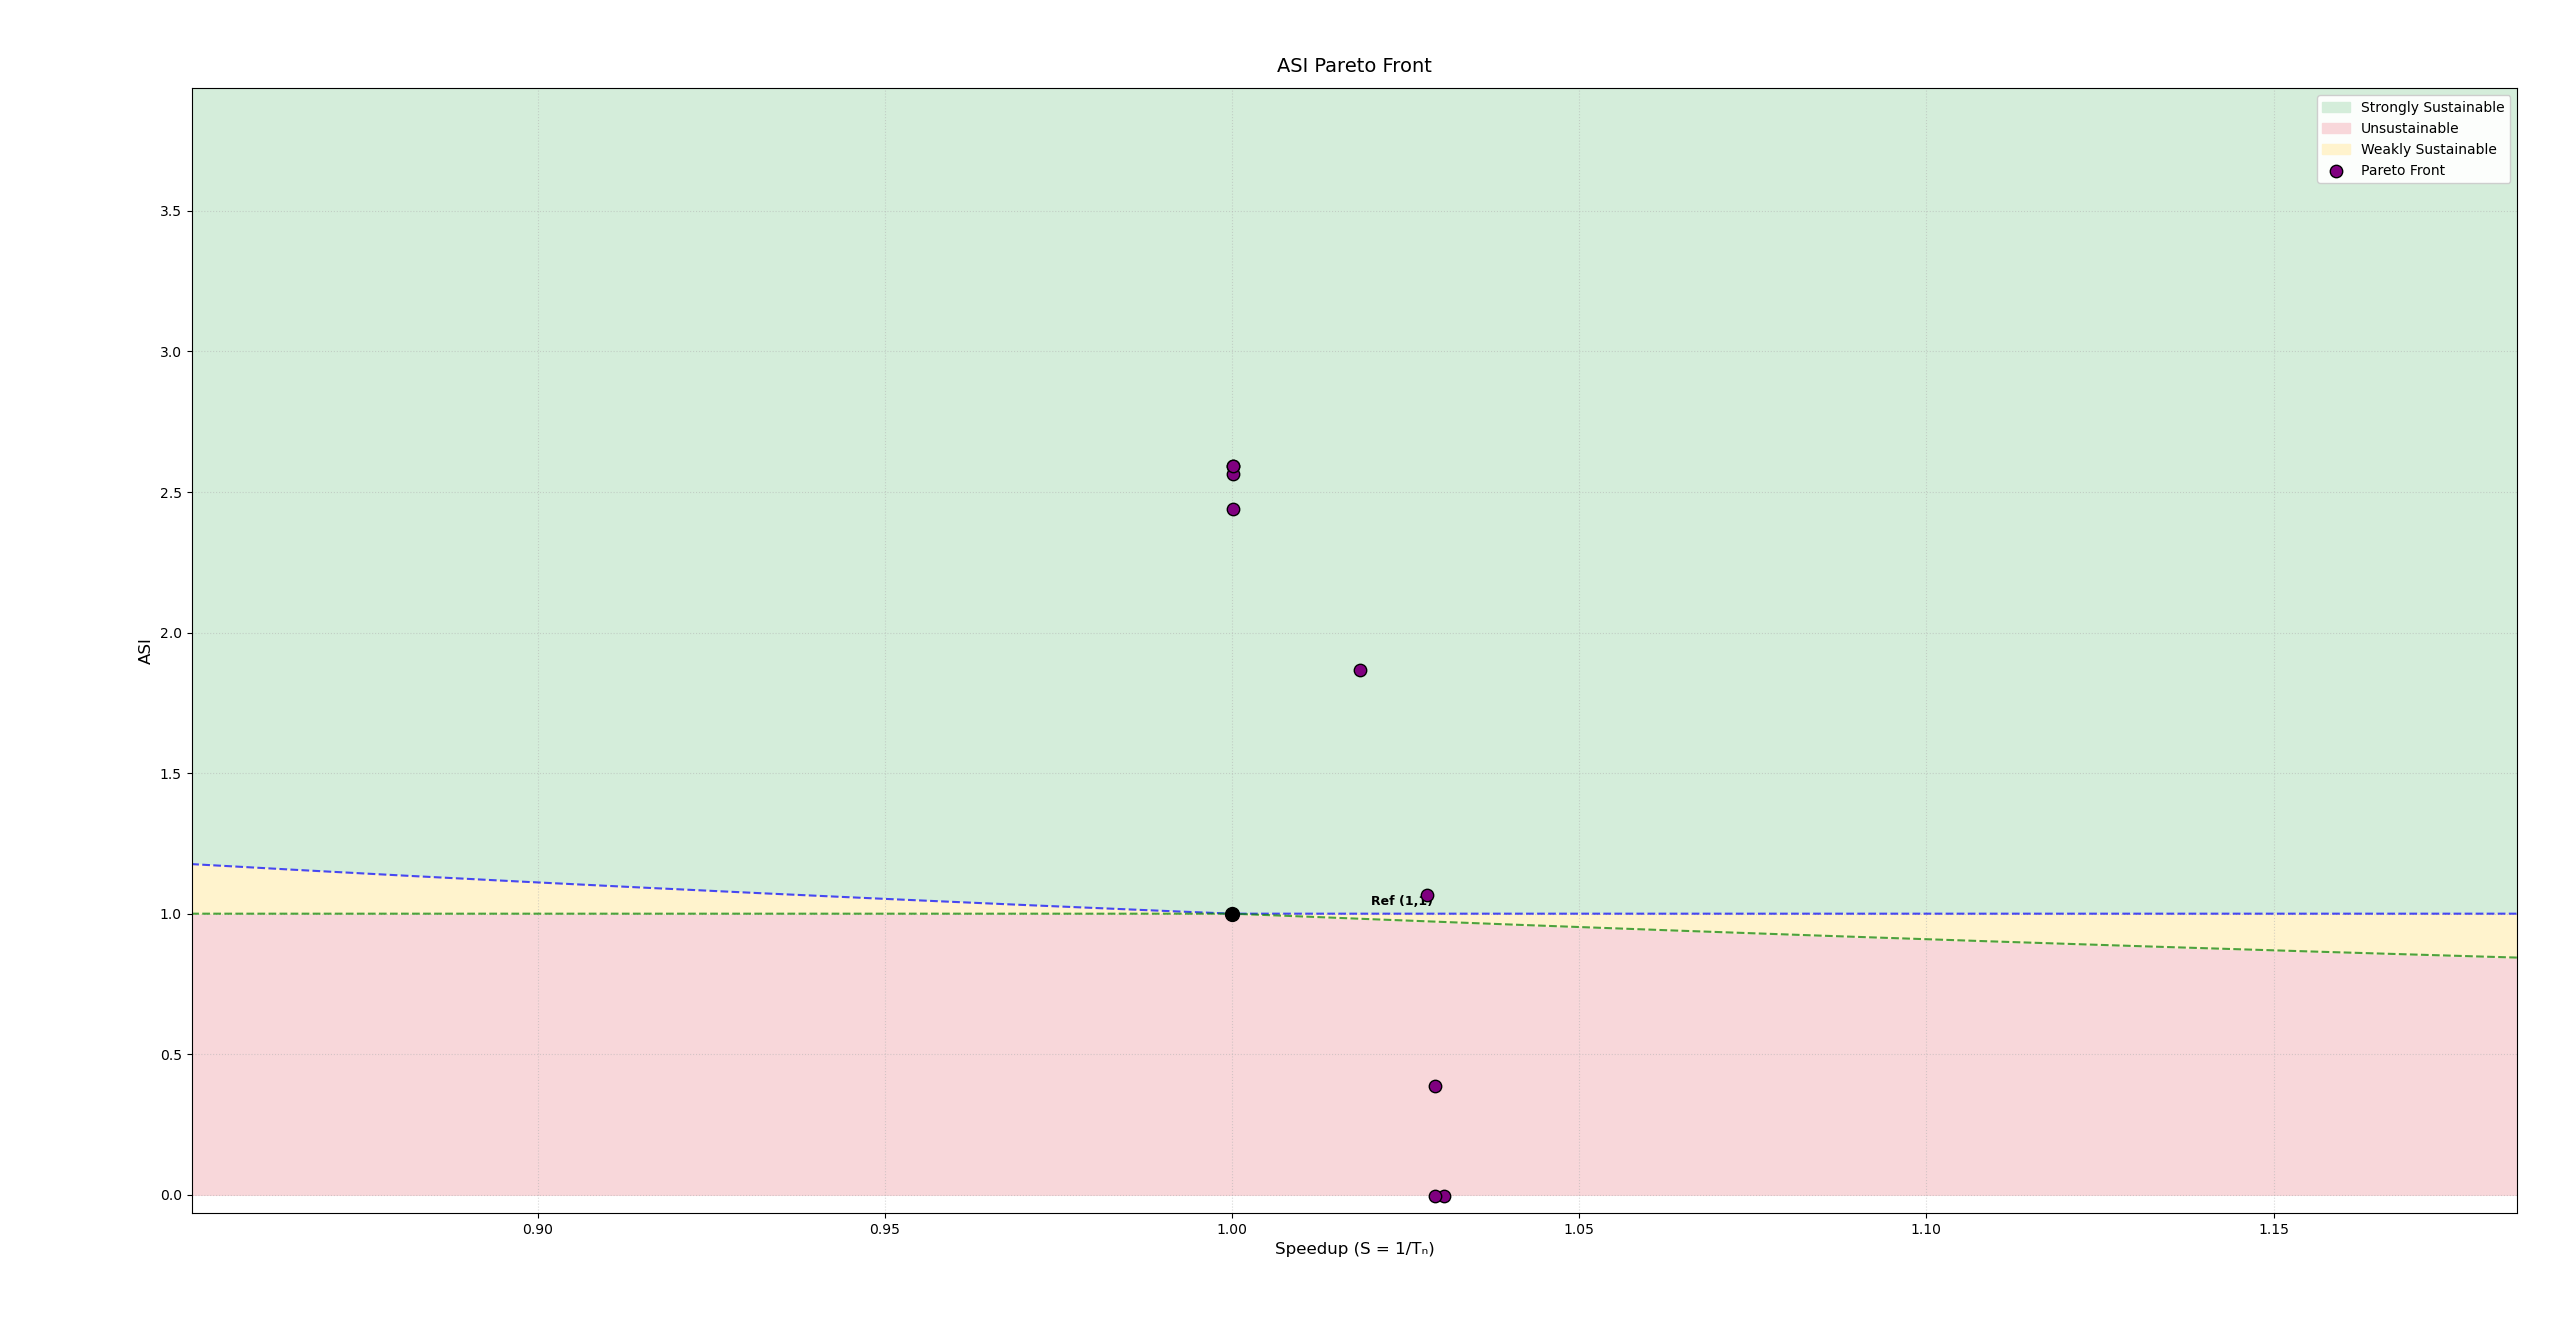
\includegraphics[width=0.48\textwidth]{../../images_results/ML2_and_CCl_mesmo.png}
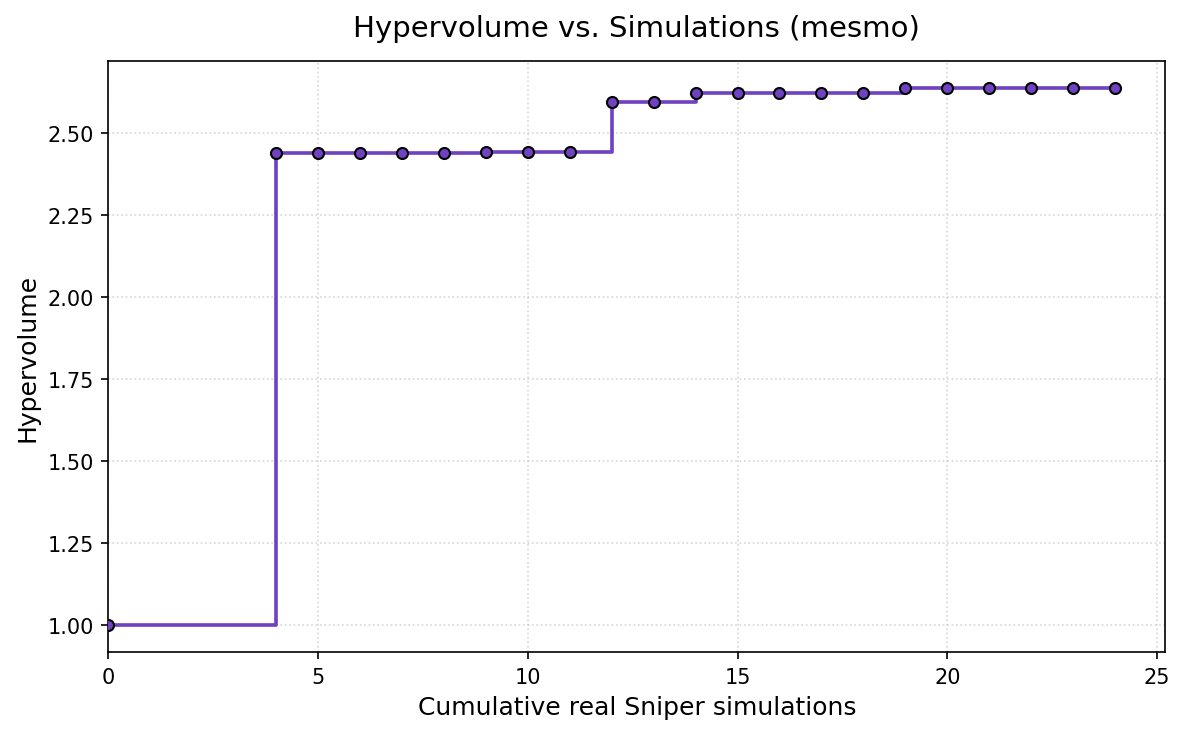
\includegraphics[width=0.48\textwidth]{../../images_results/ML2_and_CCl_mesmo_hv_vs_sims.png}
\end{figure}

\textbf{Result:}
\newline
Total sniper runs: 24
\newline
Final hypervolume: 2.6384

\textbf{Front:}

\begin{table}[H]
\centering
\resizebox{\textwidth}{!}{%
\begin{tabular}{lllllllllllllllllll}
\toprule
bpt & l1da & l1d & l1ia & l1i & l2a & l2 & l3a & l3 & nnbl & nnlr & robc & robd & robw & ASI & Speedup & Area & PeakPow & Region \\
\midrule
pentium\_m & 8 & 64 & 4 & 16 & 8 & 512 & 4 & 1024 &  &  & 8 & 10 & 1024 & -0.0056 & 1.0305 & 239.58 & 2631.93 & Unsustainable \\
pentium\_m & 8 & 16 & 4 & 16 & 8 & 512 & 4 & 1024 &  &  & 8 & 10 & 1024 & -0.0054 & 1.0293 & 238.13 & 2631.81 & Unsustainable \\
tage & 4 & 32 & 4 & 64 & 8 & 512 & 8 & 2048 &  &  & 8 & 4 & 512 & 0.3855 & 1.0293 & 57.08 & 96.36 & Unsustainable \\
nn & 8 & 16 & 4 & 16 & 8 & 512 & 8 & 2048 & 32 & 0.0005 & 2 & 2 & 1024 & 1.0671 & 1.0281 & 53.81 & 35.68 & Strongly Sust. \\
tage & 4 & 32 & 4 & 64 & 8 & 512 & 8 & 2048 &  &  & 8 & 4 & 16 & 1.8672 & 1.0185 & 49.44 & 21.06 & Strongly Sust. \\
pentium\_m & 4 & 16 & 8 & 16 & 4 & 256 & 4 & 2048 &  &  & 2 & 2 & 256 & 2.4405 & 1.0001 & 42.61 & 16.90 & Strongly Sust. \\
pentium\_m & 4 & 16 & 4 & 64 & 4 & 256 & 4 & 2048 &  &  & 2 & 2 & 256 & 2.5637 & 1.0001 & 41.82 & 16.18 & Strongly Sust. \\
pentium\_m & 4 & 16 & 4 & 16 & 4 & 256 & 4 & 2048 &  &  & 8 & 2 & 256 & 2.5931 & 1.0001 & 40.99 & 16.09 & Strongly Sust. \\
pentium\_m & 4 & 16 & 4 & 16 & 4 & 256 & 4 & 2048 &  &  & 2 & 2 & 256 & 2.5931 & 1.0001 & 40.99 & 16.09 & Strongly Sust. \\
\bottomrule
\end{tabular}
}
\end{table}

\subsubsection{hyperparameter settings 2}

hyperparameter settings: 400 candidate samples are used and 7 initial configurations have been run.
\begin{itemize}

\item 20 iterations

\begin{figure}[H]
\centering
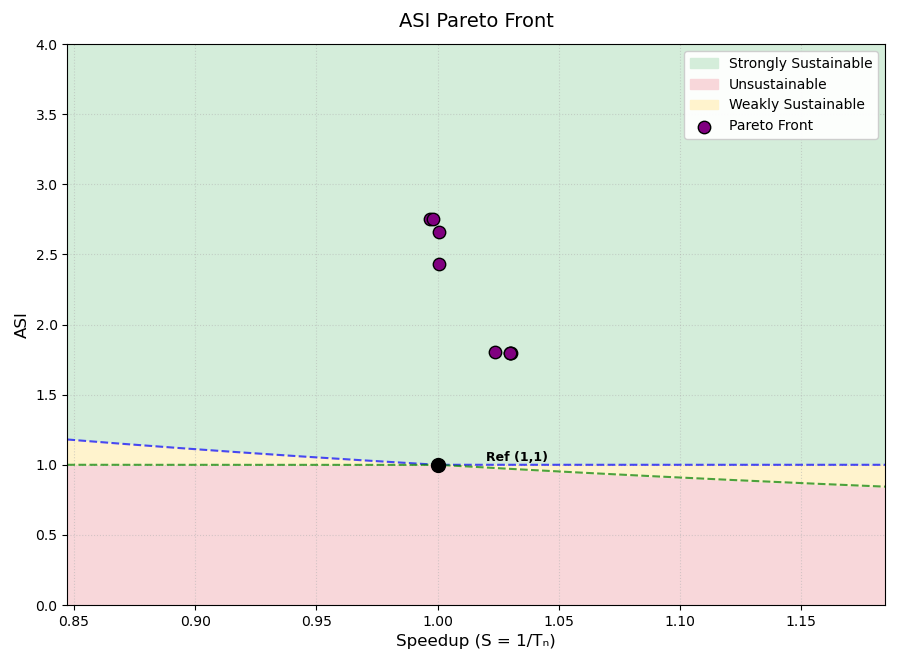
\includegraphics[width=0.48\textwidth]{../../images_results/ML2_and_CCl_mesmo_400.png}
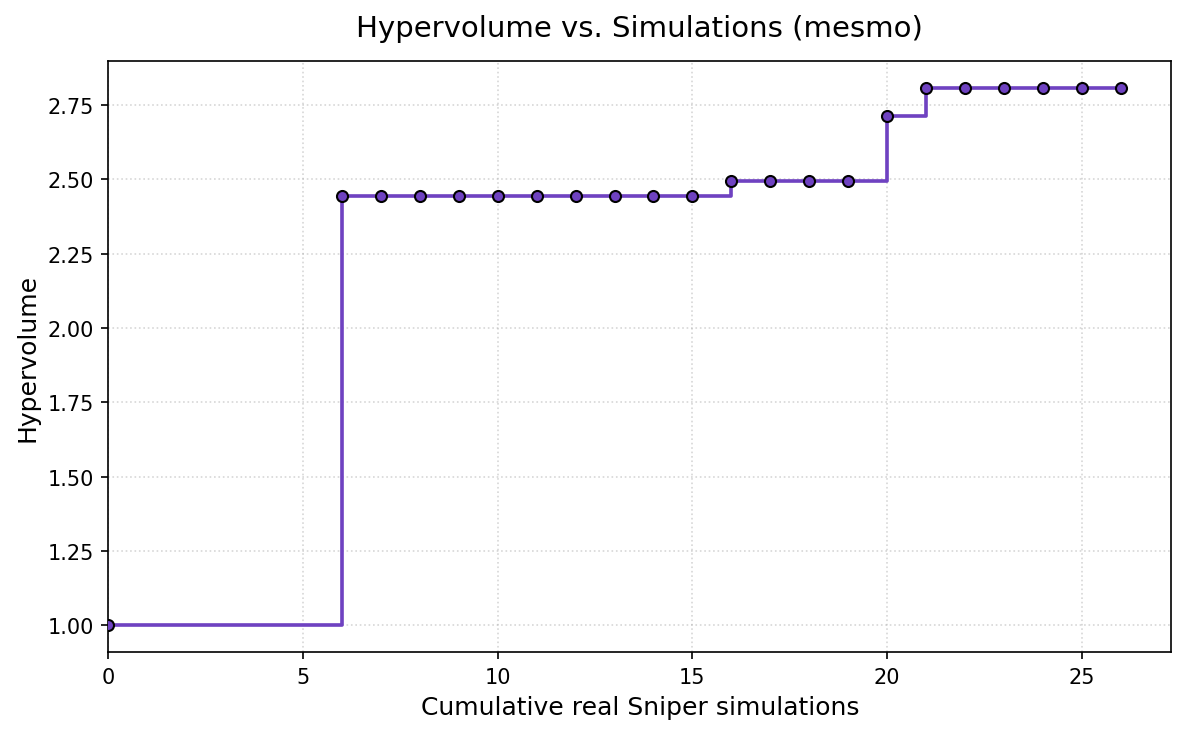
\includegraphics[width=0.48\textwidth]{../../images_results/ML2_and_CCl_mesmo_400_hv_vs_sims.png}
\end{figure}

\textbf{Result:}
\newline
Total sniper runs: 26
\newline
Final hypervolume: 2.8076

\textbf{Front:}

\begin{table}[H]
\centering
\resizebox{\textwidth}{!}{%
\begin{tabular}{lllllllllllllllllllll}
\toprule
bpt & bp & l1da & l1d & l1ia & l1i & l2a & l2 & l3a & l3 & nhist & nnbl & nnlr & robc & robd & robw & ASI & Speedup & Area & PeakPow & Region \\
\midrule
pentium\_m &  & 8 & 64 & 4 & 32 & 4 & 512 & 4 & 4096 &  &  &  & 2 & 2 & 256 & 1.7997 & 1.0301 & 65.13 & 19.37 & Strongly Sust. \\
a53 & 512 & 8 & 64 & 4 & 32 & 4 & 512 & 4 & 4096 & 4 &  &  & 2 & 2 & 256 & 1.7998 & 1.0298 & 65.13 & 19.37 & Strongly Sust. \\
a53 & 512 & 8 & 64 & 4 & 32 & 4 & 512 & 4 & 4096 & 4 &  &  & 10 & 2 & 256 & 1.7998 & 1.0298 & 65.13 & 19.37 & Strongly Sust. \\
nn &  & 8 & 64 & 4 & 32 & 4 & 512 & 4 & 4096 &  & 16 & 0.001 & 2 & 2 & 256 & 1.8013 & 1.0235 & 65.13 & 19.35 & Strongly Sust. \\
pentium\_m &  & 4 & 32 & 8 & 16 & 4 & 256 & 4 & 2048 &  &  &  & 2 & 2 & 256 & 2.4315 & 1.0005 & 42.80 & 16.94 & Strongly Sust. \\
pentium\_m &  & 4 & 32 & 8 & 16 & 4 & 256 & 4 & 1024 &  &  &  & 2 & 2 & 256 & 2.6597 & 1.0005 & 35.85 & 16.23 & Strongly Sust. \\
nn &  & 4 & 32 & 8 & 16 & 4 & 256 & 4 & 1024 &  & 16 & 0.005 & 2 & 2 & 32 & 2.7519 & 0.9982 & 35.61 & 15.71 & Strongly Sust. \\
pentium\_m &  & 4 & 32 & 8 & 16 & 4 & 256 & 4 & 1024 &  &  &  & 2 & 2 & 32 & 2.7531 & 0.9967 & 35.61 & 15.71 & Strongly Sust. \\
\bottomrule
\end{tabular}
}
\end{table}

\item 30 iterations

\begin{figure}[H]
\centering
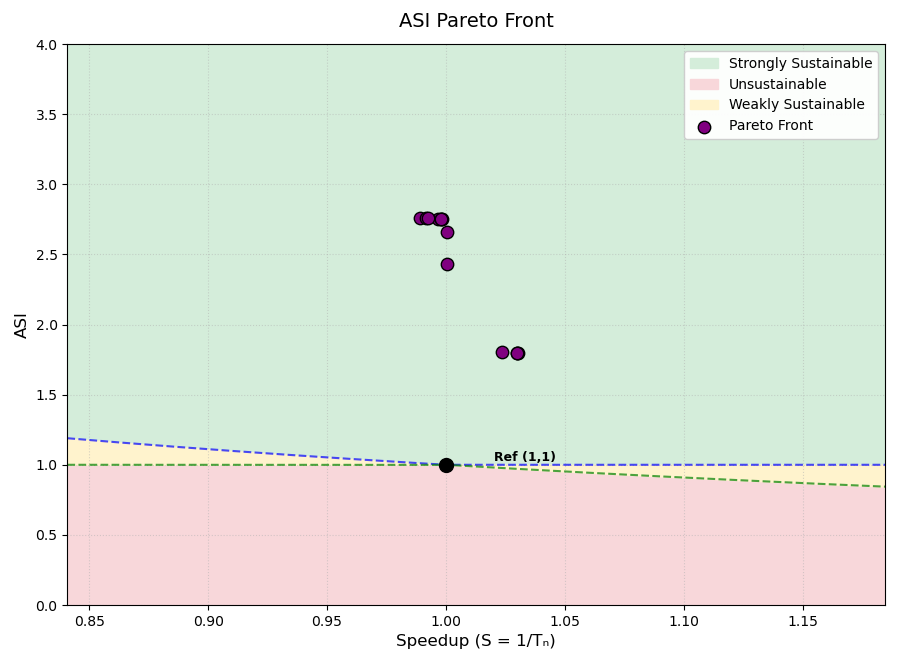
\includegraphics[width=0.48\textwidth]{../../images_results/ML2_and_CCl_mesmo_400_30iters.png}
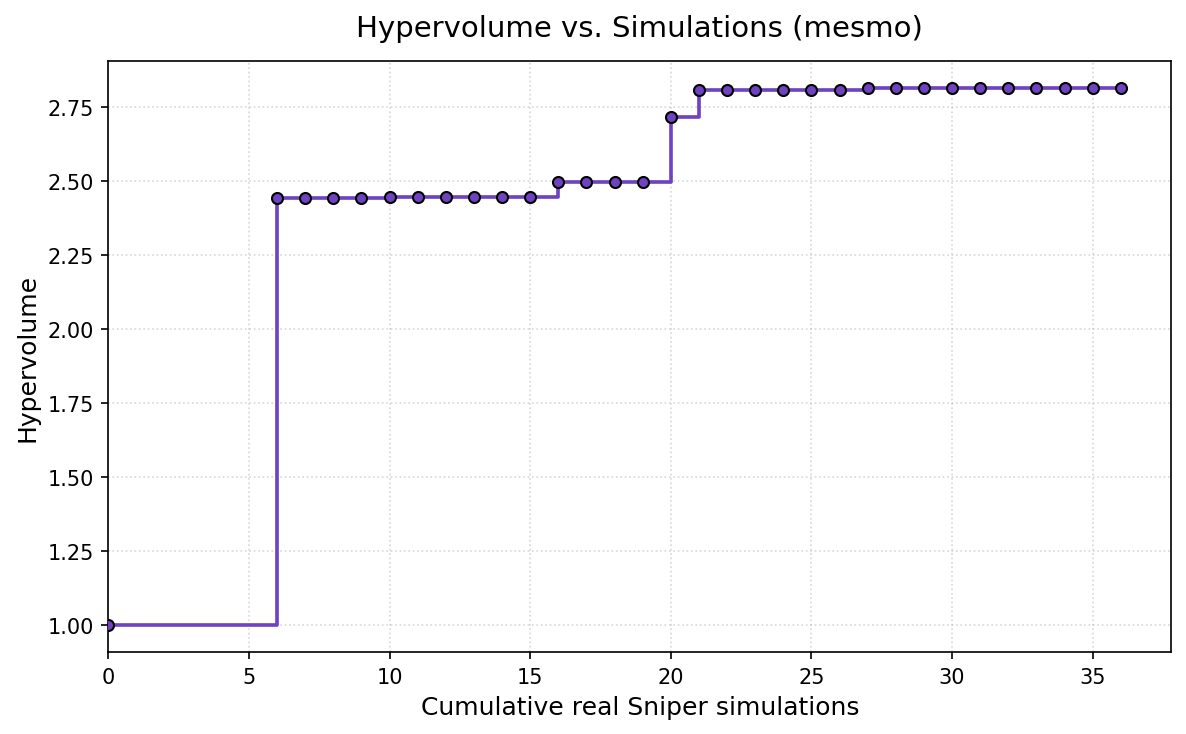
\includegraphics[width=0.48\textwidth]{../../images_results/ML2_and_CCl_mesmo_400_30iters_hv_vs_sims.png}
\end{figure}

\textbf{Result:}
\newline
Total sniper runs: 36
\newline
Final hypervolume: 2.8132

\textbf{Front:}

\begin{table}[H]
\centering
\resizebox{\textwidth}{!}{%
\begin{tabular}{lllllllllllllllllllll}
\toprule
bpt & bp & l1da & l1d & l1ia & l1i & l2a & l2 & l3a & l3 & nhist & nnbl & nnlr & robc & robd & robw & ASI & Speedup & Area & PeakPow & Region \\
\midrule
pentium\_m &  & 8 & 64 & 4 & 32 & 4 & 512 & 4 & 4096 &  &  &  & 2 & 2 & 256 & 1.7997 & 1.0301 & 65.13 & 19.37 & Strongly Sust. \\
a53 & 512 & 8 & 64 & 4 & 32 & 4 & 512 & 4 & 4096 & 4 &  &  & 2 & 2 & 256 & 1.7998 & 1.0298 & 65.13 & 19.37 & Strongly Sust. \\
a53 & 512 & 8 & 64 & 4 & 32 & 4 & 512 & 4 & 4096 & 4 &  &  & 10 & 2 & 256 & 1.7998 & 1.0298 & 65.13 & 19.37 & Strongly Sust. \\
nn &  & 8 & 64 & 4 & 32 & 4 & 512 & 4 & 4096 &  & 16 & 0.001 & 2 & 2 & 256 & 1.8013 & 1.0235 & 65.13 & 19.35 & Strongly Sust. \\
pentium\_m &  & 4 & 32 & 8 & 16 & 4 & 256 & 4 & 2048 &  &  &  & 2 & 2 & 256 & 2.4315 & 1.0005 & 42.80 & 16.94 & Strongly Sust. \\
pentium\_m &  & 4 & 32 & 8 & 16 & 4 & 256 & 4 & 1024 &  &  &  & 2 & 2 & 256 & 2.6597 & 1.0005 & 35.85 & 16.23 & Strongly Sust. \\
nn &  & 4 & 32 & 8 & 16 & 4 & 256 & 4 & 1024 &  & 16 & 0.005 & 2 & 2 & 32 & 2.7519 & 0.9982 & 35.61 & 15.71 & Strongly Sust. \\
a53 & 2048 & 4 & 32 & 8 & 16 & 4 & 256 & 4 & 1024 & 4 &  &  & 2 & 2 & 32 & 2.7520 & 0.9980 & 35.61 & 15.71 & Strongly Sust. \\
tage &  & 4 & 32 & 8 & 16 & 4 & 256 & 4 & 1024 &  &  &  & 2 & 2 & 32 & 2.7522 & 0.9978 & 35.61 & 15.71 & Strongly Sust. \\
pentium\_m &  & 4 & 32 & 8 & 16 & 4 & 256 & 4 & 1024 &  &  &  & 2 & 2 & 32 & 2.7531 & 0.9967 & 35.61 & 15.71 & Strongly Sust. \\
a53 & 1024 & 4 & 32 & 8 & 16 & 4 & 256 & 4 & 1024 & 2 &  &  & 2 & 2 & 32 & 2.7567 & 0.9923 & 35.61 & 15.68 & Strongly Sust. \\
nn &  & 4 & 32 & 8 & 16 & 4 & 256 & 4 & 1024 &  & 64 & 0.0005 & 2 & 2 & 32 & 2.7573 & 0.9915 & 35.61 & 15.68 & Strongly Sust. \\
nn &  & 4 & 32 & 8 & 16 & 4 & 256 & 4 & 1024 &  & 64 & 0.005 & 2 & 2 & 32 & 2.7587 & 0.9892 & 35.61 & 15.67 & Strongly Sust. \\
\bottomrule
\end{tabular}
}
\end{table}

\item 40 iterations

\begin{figure}[H]
\centering
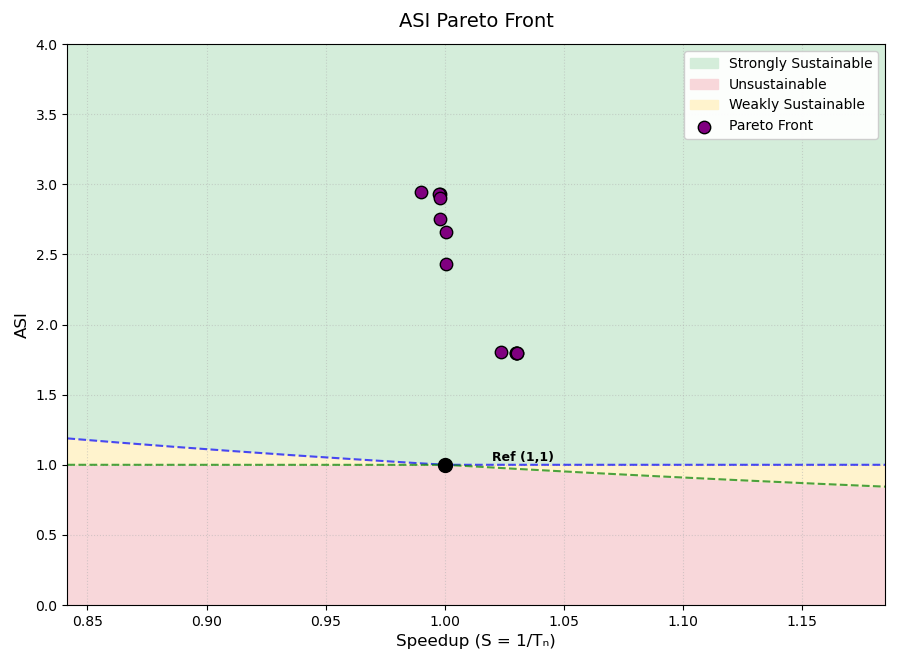
\includegraphics[width=0.48\textwidth]{../../images_results/ML2_and_CCl_mesmo_400_40iters.png}
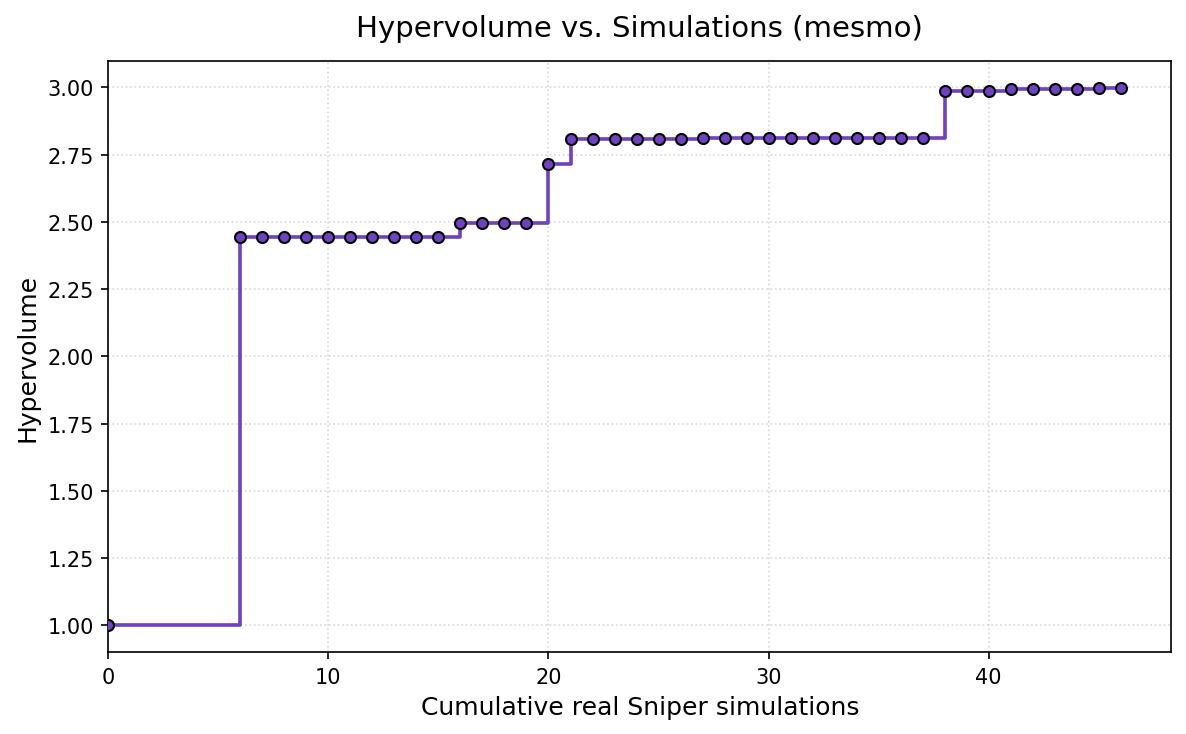
\includegraphics[width=0.48\textwidth]{../../images_results/ML2_and_CCl_mesmo_400_40iters_hv_vs_sims.png}
\end{figure}

\textbf{Result:}
\newline
Total sniper runs: 46
\newline
Final hypervolume: 2.9982

\textbf{Front:}

\begin{table}[H]
\centering
\resizebox{\textwidth}{!}{%
\begin{tabular}{lllllllllllllllllllll}
\toprule
bpt & bp & l1da & l1d & l1ia & l1i & l2a & l2 & l3a & l3 & nhist & nnbl & nnlr & robc & robd & robw & ASI & Speedup & Area & PeakPow & Region \\
\midrule
pentium\_m &  & 8 & 64 & 4 & 32 & 4 & 512 & 4 & 4096 &  &  &  & 8 & 2 & 256 & 1.7997 & 1.0302 & 65.13 & 19.37 & Strongly Sust. \\
pentium\_m &  & 8 & 64 & 4 & 32 & 4 & 512 & 4 & 4096 &  &  &  & 2 & 2 & 256 & 1.7997 & 1.0301 & 65.13 & 19.37 & Strongly Sust. \\
a53 & 512 & 8 & 64 & 4 & 32 & 4 & 512 & 4 & 4096 & 4 &  &  & 2 & 2 & 256 & 1.7998 & 1.0298 & 65.13 & 19.37 & Strongly Sust. \\
a53 & 512 & 8 & 64 & 4 & 32 & 4 & 512 & 4 & 4096 & 4 &  &  & 10 & 2 & 256 & 1.7998 & 1.0298 & 65.13 & 19.37 & Strongly Sust. \\
nn &  & 8 & 64 & 4 & 32 & 4 & 512 & 4 & 4096 &  & 16 & 0.001 & 2 & 2 & 256 & 1.8013 & 1.0235 & 65.13 & 19.35 & Strongly Sust. \\
pentium\_m &  & 4 & 32 & 8 & 16 & 4 & 256 & 4 & 2048 &  &  &  & 2 & 2 & 256 & 2.4315 & 1.0005 & 42.80 & 16.94 & Strongly Sust. \\
pentium\_m &  & 4 & 32 & 8 & 16 & 4 & 256 & 4 & 1024 &  &  &  & 2 & 2 & 256 & 2.6597 & 1.0005 & 35.85 & 16.23 & Strongly Sust. \\
nn &  & 4 & 32 & 8 & 16 & 4 & 256 & 4 & 1024 &  & 16 & 0.005 & 2 & 2 & 32 & 2.7519 & 0.9982 & 35.61 & 15.71 & Strongly Sust. \\
a53 & 2048 & 4 & 32 & 4 & 64 & 4 & 256 & 4 & 1024 & 4 &  &  & 2 & 2 & 32 & 2.8998 & 0.9981 & 34.82 & 14.99 & Strongly Sust. \\
a53 & 2048 & 4 & 32 & 4 & 16 & 4 & 256 & 4 & 1024 & 4 &  &  & 2 & 2 & 32 & 2.9337 & 0.9980 & 34.00 & 14.89 & Strongly Sust. \\
a53 & 1024 & 4 & 32 & 4 & 16 & 4 & 256 & 4 & 1024 & 4 &  &  & 2 & 2 & 32 & 2.9341 & 0.9975 & 34.00 & 14.89 & Strongly Sust. \\
a53 & 2048 & 4 & 32 & 4 & 64 & 4 & 256 & 4 & 1024 & 4 &  &  & 2 & 2 & 16 & 2.9440 & 0.9902 & 34.74 & 14.77 & Strongly Sust. \\
\bottomrule
\end{tabular}
}
\end{table}

\item 50 iterations

Mistake with automatic plotting, but conclusion is that hypervolume keeps increasing.

\textbf{Result:}
\newline
Total sniper runs: 56
\newline
Final hypervolume: 3.0285

\textbf{Front:}

\begin{table}[H]
\centering
\resizebox{\textwidth}{!}{%
\begin{tabular}{lllllllllllllllllllll}
\toprule
bpt & bp & l1da & l1d & l1ia & l1i & l2a & l2 & l3a & l3 & nhist & nnbl & nnlr & robc & robd & robw & ASI & Speedup & Area & PeakPow & Region \\
\midrule
tage &  & 8 & 64 & 8 & 16 & 4 & 512 & 4 & 4096 &  &  &  & 8 & 2 & 1024 & 0.8705 & 1.0304 & 70.96 & 38.15 & Unsustainable \\
pentium\_m &  & 8 & 64 & 8 & 32 & 8 & 512 & 16 & 2048 &  &  &  & 10 & 2 & 512 & 1.4025 & 1.0302 & 56.00 & 26.71 & Strongly Sust. \\
pentium\_m &  & 8 & 64 & 8 & 32 & 8 & 512 & 16 & 2048 &  &  &  & 8 & 2 & 512 & 1.4025 & 1.0302 & 56.00 & 26.71 & Strongly Sust. \\
pentium\_m &  & 8 & 64 & 4 & 32 & 4 & 512 & 4 & 4096 &  &  &  & 8 & 2 & 256 & 1.7997 & 1.0302 & 65.13 & 19.37 & Strongly Sust. \\
pentium\_m &  & 8 & 64 & 4 & 32 & 4 & 512 & 4 & 4096 &  &  &  & 2 & 2 & 256 & 1.7997 & 1.0301 & 65.13 & 19.37 & Strongly Sust. \\
pentium\_m &  & 8 & 64 & 8 & 32 & 8 & 512 & 16 & 2048 &  &  &  & 8 & 2 & 128 & 2.0450 & 1.0299 & 54.39 & 18.54 & Strongly Sust. \\
pentium\_m &  & 4 & 32 & 8 & 16 & 4 & 256 & 4 & 2048 &  &  &  & 2 & 2 & 256 & 2.4315 & 1.0005 & 42.80 & 16.94 & Strongly Sust. \\
pentium\_m &  & 4 & 32 & 8 & 16 & 4 & 256 & 4 & 1024 &  &  &  & 2 & 2 & 256 & 2.6597 & 1.0005 & 35.85 & 16.23 & Strongly Sust. \\
nn &  & 4 & 32 & 8 & 16 & 4 & 256 & 4 & 1024 &  & 16 & 0.005 & 2 & 2 & 32 & 2.7519 & 0.9982 & 35.61 & 15.71 & Strongly Sust. \\
a53 & 2048 & 4 & 32 & 4 & 64 & 4 & 256 & 4 & 1024 & 4 &  &  & 2 & 2 & 32 & 2.8998 & 0.9981 & 34.82 & 14.99 & Strongly Sust. \\
a53 & 2048 & 4 & 32 & 4 & 16 & 4 & 256 & 4 & 1024 & 4 &  &  & 2 & 2 & 32 & 2.9337 & 0.9980 & 34.00 & 14.89 & Strongly Sust. \\
a53 & 1024 & 4 & 32 & 4 & 16 & 4 & 256 & 4 & 1024 & 4 &  &  & 2 & 2 & 32 & 2.9341 & 0.9975 & 34.00 & 14.89 & Strongly Sust. \\
a53 & 2048 & 4 & 32 & 4 & 64 & 4 & 256 & 4 & 1024 & 4 &  &  & 2 & 2 & 16 & 2.9440 & 0.9902 & 34.74 & 14.77 & Strongly Sust. \\
pentium\_m &  & 4 & 32 & 4 & 64 & 4 & 256 & 4 & 1024 &  &  &  & 2 & 2 & 16 & 2.9461 & 0.9874 & 34.74 & 14.76 & Strongly Sust. \\
nn &  & 4 & 32 & 4 & 64 & 4 & 256 & 4 & 1024 &  & 64 & 0.001 & 2 & 2 & 16 & 2.9679 & 0.9577 & 34.74 & 14.65 & Strongly Sust. \\
\bottomrule
\end{tabular}
}
\end{table}

\item 60 iterations

\textbf{Result:}
\newline
Total sniper runs: 66
\newline
Final hypervolume: 3.0375

\textbf{Front:}

\begin{table}[H]
\centering
\resizebox{\textwidth}{!}{%
\begin{tabular}{lllllllllllllllllllll}
\toprule
bpt & bp & l1da & l1d & l1ia & l1i & l2a & l2 & l3a & l3 & nhist & nnbl & nnlr & robc & robd & robw & ASI & Speedup & Area & PeakPow & Region \\
\midrule
tage &  & 8 & 64 & 8 & 16 & 4 & 512 & 4 & 4096 &  &  &  & 8 & 2 & 1024 & 0.8705 & 1.0304 & 70.96 & 38.15 & Unsustainable \\
pentium\_m &  & 8 & 64 & 8 & 32 & 8 & 512 & 16 & 2048 &  &  &  & 10 & 2 & 512 & 1.4025 & 1.0302 & 56.00 & 26.71 & Strongly Sust. \\
pentium\_m &  & 8 & 64 & 8 & 32 & 8 & 512 & 16 & 2048 &  &  &  & 8 & 2 & 512 & 1.4025 & 1.0302 & 56.00 & 26.71 & Strongly Sust. \\
pentium\_m &  & 8 & 64 & 4 & 32 & 4 & 512 & 4 & 4096 &  &  &  & 8 & 2 & 256 & 1.7997 & 1.0302 & 65.13 & 19.37 & Strongly Sust. \\
pentium\_m &  & 8 & 64 & 4 & 32 & 4 & 512 & 4 & 4096 &  &  &  & 2 & 2 & 256 & 1.7997 & 1.0301 & 65.13 & 19.37 & Strongly Sust. \\
pentium\_m &  & 8 & 64 & 8 & 32 & 8 & 512 & 16 & 2048 &  &  &  & 8 & 2 & 128 & 2.0450 & 1.0299 & 54.39 & 18.54 & Strongly Sust. \\
a53 & 2048 & 8 & 32 & 4 & 64 & 4 & 512 & 16 & 1024 & 4 &  &  & 8 & 2 & 64 & 2.3621 & 1.0287 & 47.90 & 16.83 & Strongly Sust. \\
pentium\_m &  & 4 & 32 & 8 & 16 & 4 & 256 & 4 & 2048 &  &  &  & 2 & 2 & 256 & 2.4315 & 1.0005 & 42.80 & 16.94 & Strongly Sust. \\
pentium\_m &  & 4 & 32 & 8 & 16 & 4 & 256 & 4 & 1024 &  &  &  & 2 & 2 & 256 & 2.6597 & 1.0005 & 35.85 & 16.23 & Strongly Sust. \\
nn &  & 4 & 32 & 8 & 16 & 4 & 256 & 4 & 1024 &  & 16 & 0.005 & 2 & 2 & 32 & 2.7519 & 0.9982 & 35.61 & 15.71 & Strongly Sust. \\
a53 & 2048 & 4 & 32 & 4 & 64 & 4 & 256 & 4 & 1024 & 4 &  &  & 2 & 2 & 32 & 2.8998 & 0.9981 & 34.82 & 14.99 & Strongly Sust. \\
a53 & 2048 & 4 & 32 & 4 & 16 & 4 & 256 & 4 & 1024 & 4 &  &  & 2 & 2 & 32 & 2.9337 & 0.9980 & 34.00 & 14.89 & Strongly Sust. \\
a53 & 1024 & 4 & 32 & 4 & 16 & 4 & 256 & 4 & 1024 & 4 &  &  & 2 & 2 & 32 & 2.9341 & 0.9975 & 34.00 & 14.89 & Strongly Sust. \\
a53 & 2048 & 4 & 32 & 4 & 64 & 4 & 256 & 4 & 1024 & 4 &  &  & 2 & 2 & 16 & 2.9440 & 0.9902 & 34.74 & 14.77 & Strongly Sust. \\
pentium\_m &  & 4 & 32 & 4 & 64 & 4 & 256 & 4 & 1024 &  &  &  & 8 & 2 & 16 & 2.9461 & 0.9874 & 34.74 & 14.76 & Strongly Sust. \\
pentium\_m &  & 4 & 32 & 4 & 64 & 4 & 256 & 4 & 1024 &  &  &  & 2 & 2 & 16 & 2.9461 & 0.9874 & 34.74 & 14.76 & Strongly Sust. \\
a53 & 512 & 4 & 32 & 4 & 64 & 4 & 256 & 4 & 1024 & 4 &  &  & 2 & 2 & 16 & 2.9463 & 0.9871 & 34.74 & 14.76 & Strongly Sust. \\
nn &  & 4 & 32 & 4 & 64 & 4 & 256 & 4 & 1024 &  & 16 & 0.001 & 10 & 2 & 16 & 2.9521 & 0.9789 & 34.74 & 14.73 & Strongly Sust. \\
nn &  & 4 & 32 & 4 & 64 & 4 & 256 & 4 & 1024 &  & 16 & 0.001 & 2 & 2 & 16 & 2.9678 & 0.9580 & 34.74 & 14.65 & Strongly Sust. \\
nn &  & 4 & 32 & 4 & 64 & 4 & 256 & 4 & 1024 &  & 64 & 0.001 & 2 & 2 & 16 & 2.9679 & 0.9577 & 34.74 & 14.65 & Strongly Sust. \\
\bottomrule
\end{tabular}
}
\end{table}
\end{itemize}
\section{ML2, CCl, MIP and EI benchmarks}

ML2: L2 resident (depending on LFSR settings) linked list traversal

CCl: Impossible control with large basic blocks (potentially larger penalty)

MIP: Large Instruction Region -- Instruction cache Misses

EI: Integer Execution -- 8 Independent computations per iteration
\subsection{MESMO}

\subsubsection{hyperparameter settings 1}

hyperparameter settings: 200 candidate samples are used and 5 initial configurations are ran. 20 iterations.

\begin{figure}[H]
\centering
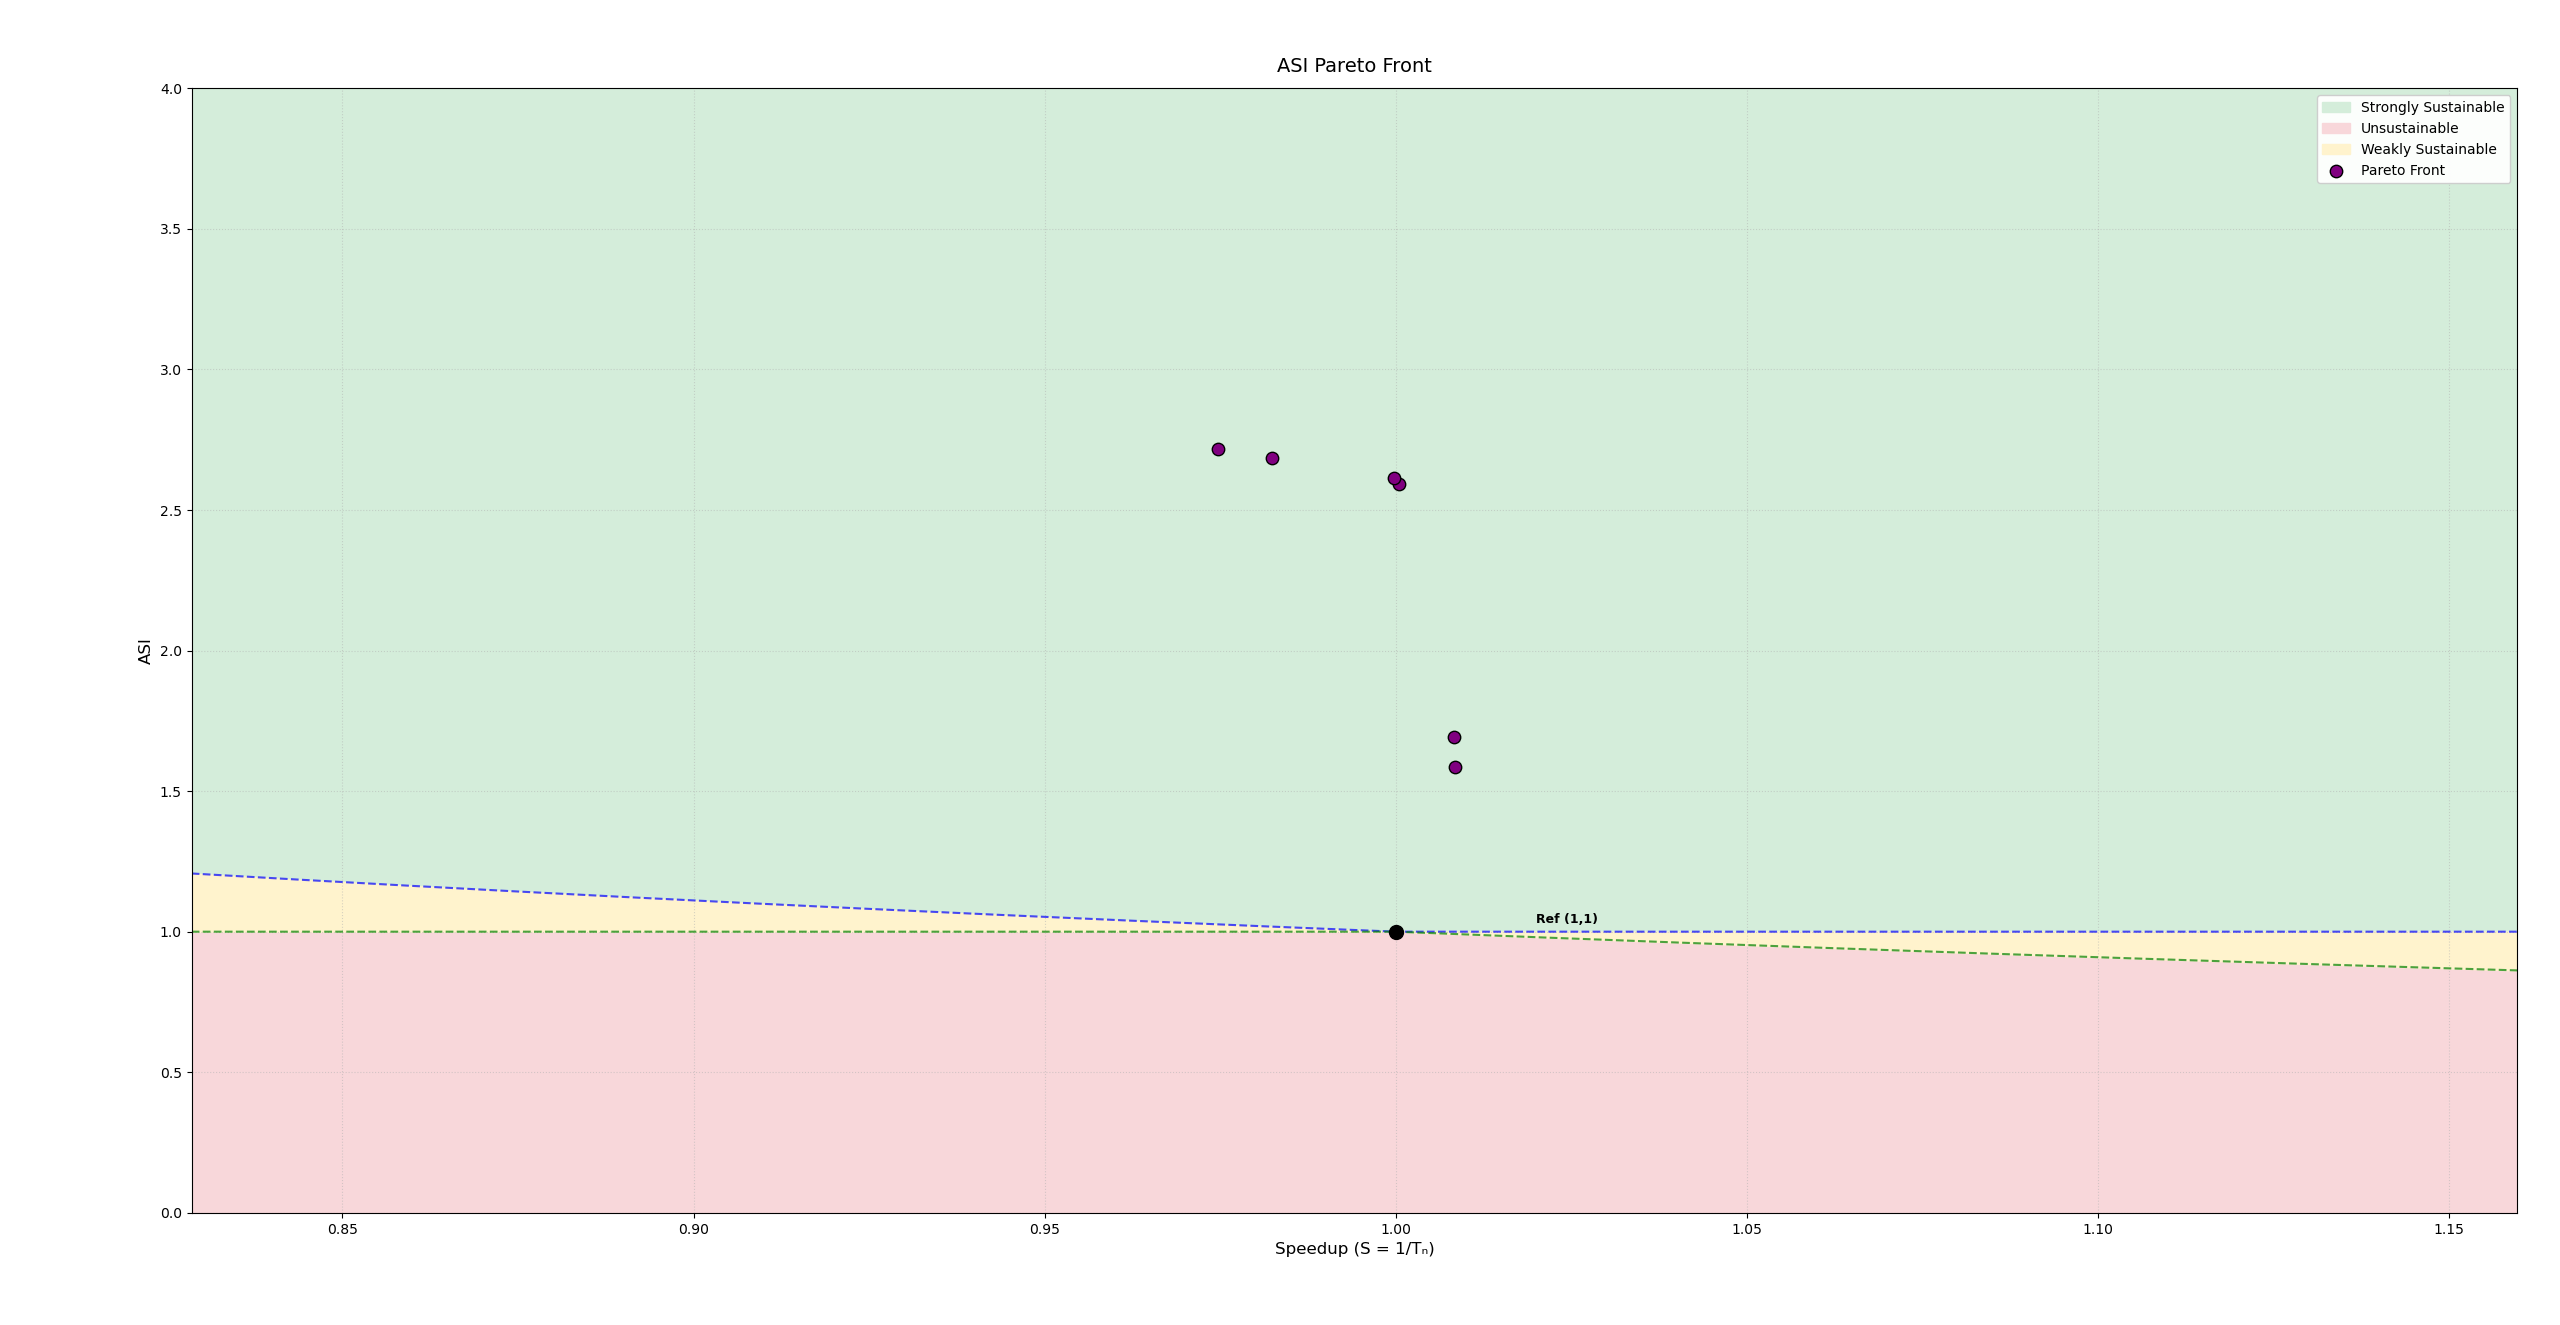
\includegraphics[width=0.48\textwidth]{../../images_results/ML2_CCl_MIP_EI_mesmo.png}
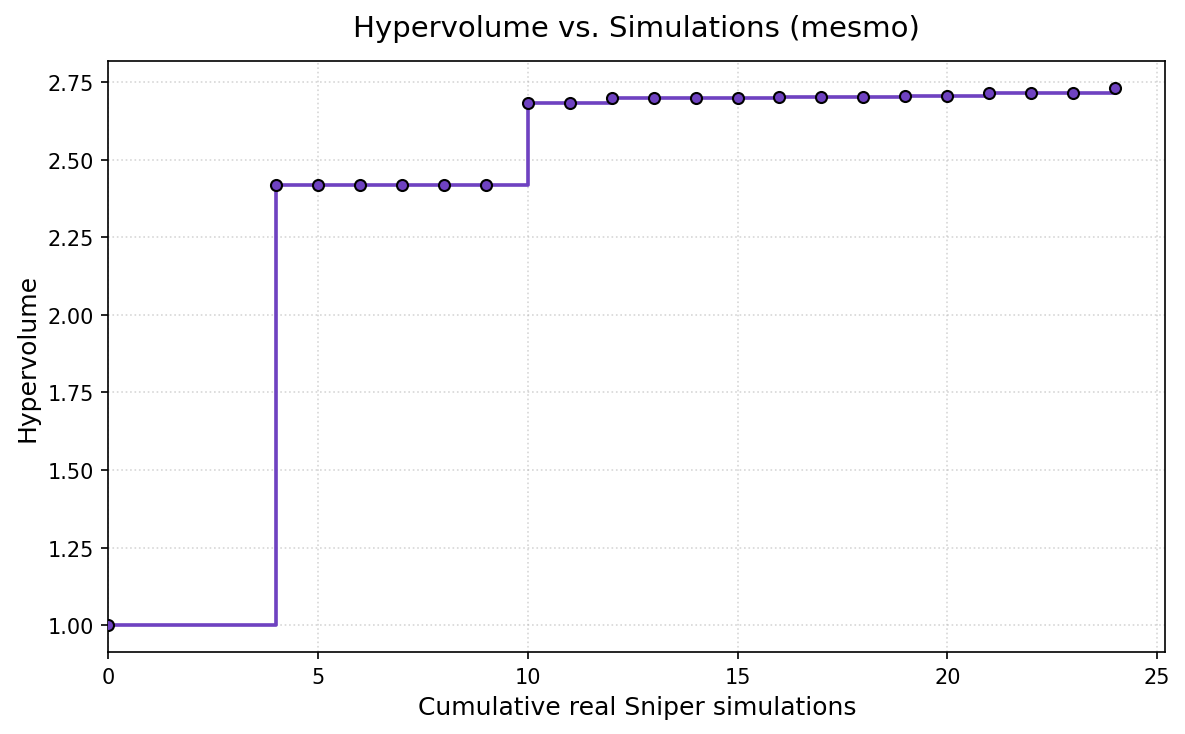
\includegraphics[width=0.48\textwidth]{../../images_results/ML2_CCl_MIP_EI_mesmo_hv_vs_sims.png}
\end{figure}

\textbf{Result:}
\newline
Total sniper runs: 24
\newline
Final hypervolume: 2.7310

\textbf{Front:}

\begin{table}[H]
\centering
\resizebox{\textwidth}{!}{%
\begin{tabular}{lllllllllllllllllll}
\toprule
bpt & l1da & l1d & l1ia & l1i & l2a & l2 & l3a & l3 & nnbl & nnlr & robc & robd & robw & ASI & Speedup & Area & PeakPow & Region \\
\midrule
pentium\_m & 4 & 64 & 4 & 32 & 8 & 512 & 8 & 2048 &  &  & 2 & 2 & 512 & 1.5862 & 1.0085 & 48.11 & 25.86 & Strongly Sust. \\
pentium\_m & 4 & 64 & 4 & 32 & 8 & 512 & 4 & 1024 &  &  & 2 & 2 & 512 & 1.6928 & 1.0083 & 42.91 & 25.13 & Strongly Sust. \\
pentium\_m & 4 & 64 & 4 & 32 & 8 & 512 & 4 & 1024 &  &  & 2 & 2 & 32 & 2.5911 & 1.0004 & 41.18 & 16.62 & Strongly Sust. \\
pentium\_m & 4 & 16 & 4 & 32 & 8 & 512 & 4 & 1024 &  &  & 2 & 2 & 32 & 2.6146 & 0.9998 & 40.81 & 16.51 & Strongly Sust. \\
nn & 8 & 16 & 4 & 32 & 8 & 256 & 4 & 1024 & 64 & 0.005 & 2 & 2 & 64 & 2.6838 & 0.9823 & 37.99 & 16.39 & Strongly Sust. \\
nn & 8 & 16 & 4 & 32 & 8 & 256 & 4 & 1024 & 64 & 0.005 & 2 & 2 & 32 & 2.7184 & 0.9747 & 37.93 & 16.19 & Strongly Sust. \\
\bottomrule
\end{tabular}
}
\end{table}

\subsubsection{hyperparameter settings 2}

hyperparameter settings: 400 candidate samples are used and 5 initial configurations are ran. 20 iterations. 4 benchmarks: ML2, CCl, MIP and EI.

\begin{figure}[H]
\centering
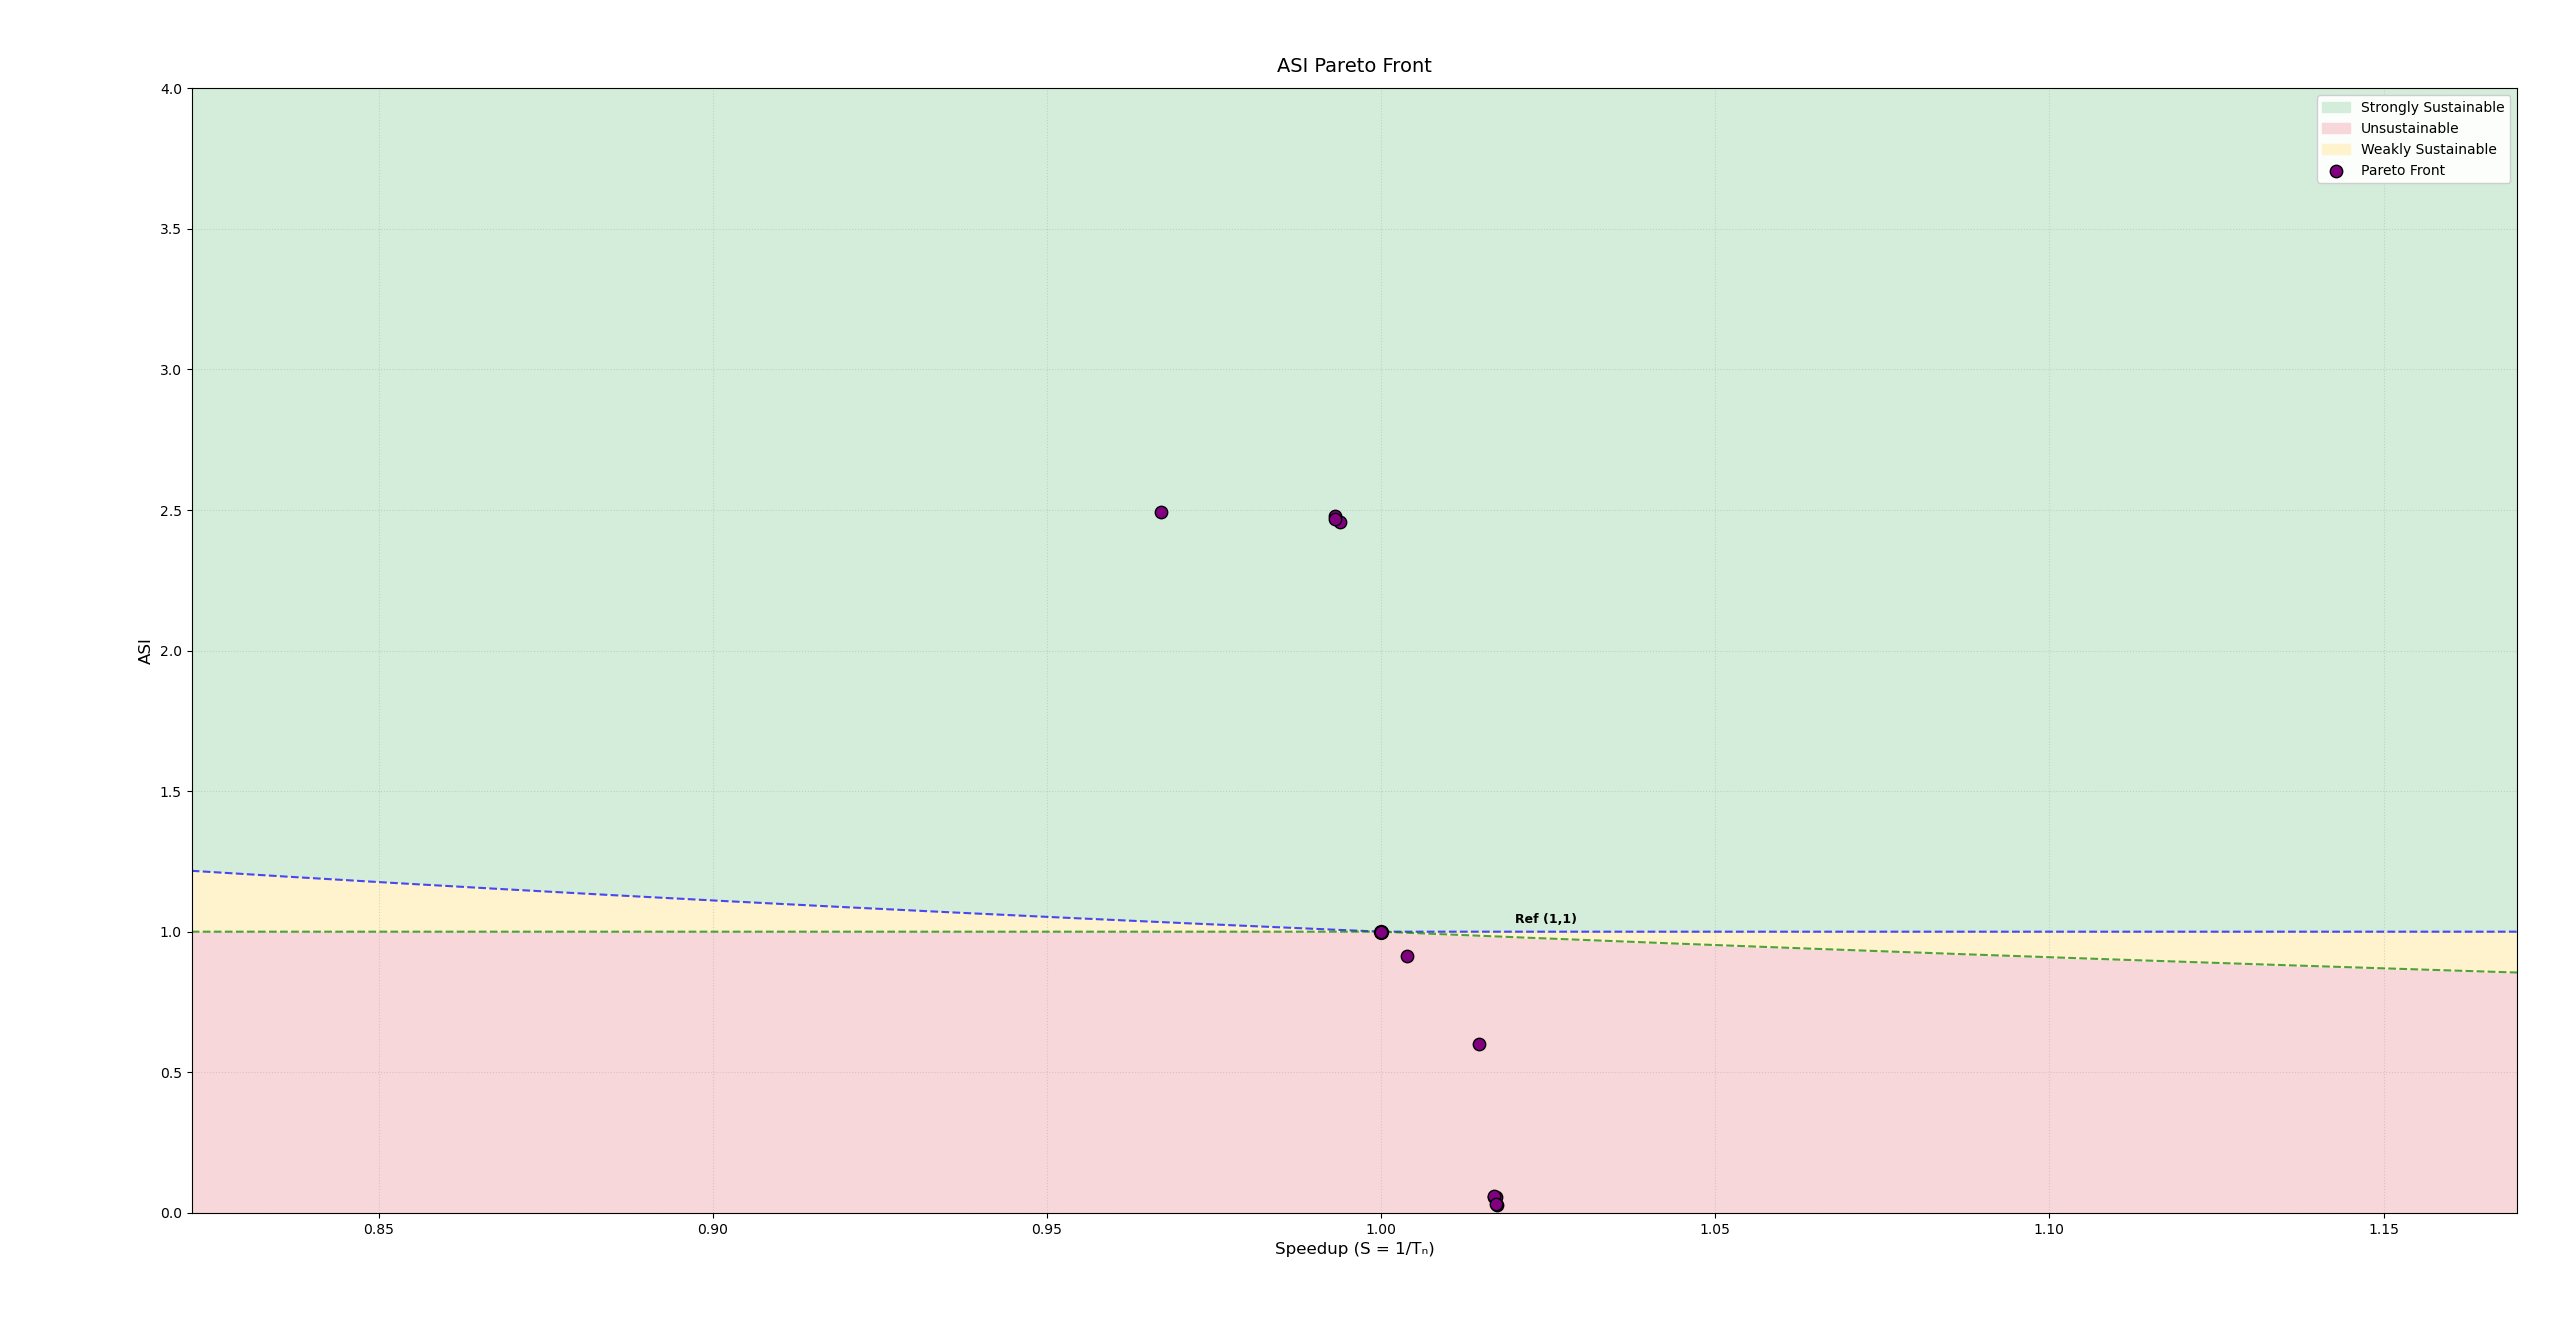
\includegraphics[width=0.48\textwidth]{../../images_results/ML2_CCl_MIP_EI_mesmo_400.png}
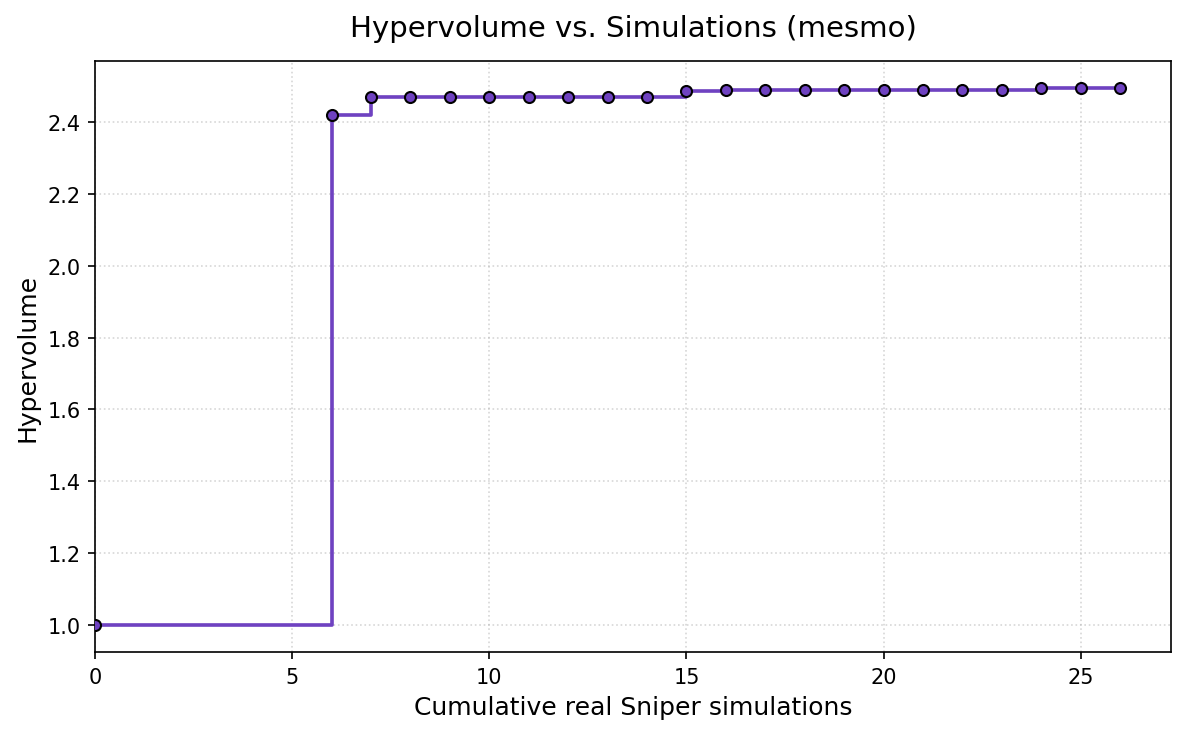
\includegraphics[width=0.48\textwidth]{../../images_results/ML2_CCl_MIP_EI_mesmo_400_hv_vs_sims.png}
\end{figure}

\textbf{Result:}
\newline
Total sniper runs: 26
\newline
Final hypervolume: 2.4945

\textbf{Front:}

\begin{table}[H]
\centering
\resizebox{\textwidth}{!}{%
\begin{tabular}{lllllllllllllllllllll}
\toprule
bpt & bp & l1da & l1d & l1ia & l1i & l2a & l2 & l3a & l3 & nhist & nnbl & nnlr & robc & robd & robw & ASI & Speedup & Area & PeakPow & Region \\
\midrule
pentium\_m &  & 4 & 64 & 4 & 16 & 8 & 512 & 8 & 4096 &  &  &  & 8 & 8 & 512 & 0.0267 & 1.0174 & 118.45 & 763.80 & Unsustainable \\
a53 & 512 & 8 & 64 & 8 & 16 & 8 & 512 & 16 & 1024 & 2 &  &  & 10 & 8 & 512 & 0.0310 & 1.0172 & 107.21 & 763.19 & Unsustainable \\
pentium\_m &  & 8 & 64 & 8 & 16 & 8 & 512 & 16 & 1024 &  &  &  & 10 & 8 & 256 & 0.0572 & 1.0171 & 83.61 & 535.26 & Unsustainable \\
a53 & 512 & 8 & 64 & 8 & 16 & 8 & 512 & 16 & 1024 & 2 &  &  & 10 & 8 & 256 & 0.0572 & 1.0170 & 83.61 & 535.26 & Unsustainable \\
a53 & 512 & 4 & 64 & 8 & 16 & 8 & 512 & 16 & 1024 & 2 &  &  & 10 & 8 & 256 & 0.0597 & 1.0170 & 79.19 & 534.47 & Unsustainable \\
pentium\_m &  & 8 & 64 & 4 & 32 & 8 & 512 & 8 & 1024 &  &  &  & 2 & 10 & 64 & 0.6014 & 1.0147 & 63.70 & 60.61 & Unsustainable \\
tage &  & 8 & 64 & 4 & 16 & 4 & 512 & 8 & 1024 &  &  &  & 10 & 8 & 32 & 0.9122 & 1.0039 & 56.76 & 42.19 & Unsustainable \\
baseline &  &  &  &  &  &  &  &  &  &  &  &  &  &  &  & 1.0000 & 1.0000 & 94.01 & 27.56 & Reference \\
pentium\_m &  & 4 & 64 & 8 & 16 & 4 & 256 & 4 & 2048 &  &  &  & 2 & 2 & 64 & 2.4560 & 0.9938 & 42.80 & 17.34 & Strongly Sust. \\
pentium\_m &  & 4 & 16 & 8 & 32 & 4 & 256 & 4 & 2048 &  &  &  & 2 & 2 & 64 & 2.4675 & 0.9931 & 42.78 & 17.26 & Strongly Sust. \\
pentium\_m &  & 4 & 16 & 8 & 16 & 4 & 256 & 4 & 2048 &  &  &  & 2 & 2 & 64 & 2.4779 & 0.9931 & 42.43 & 17.23 & Strongly Sust. \\
nn &  & 4 & 16 & 8 & 32 & 4 & 256 & 4 & 2048 &  & 64 & 0.005 & 2 & 2 & 64 & 2.4940 & 0.9671 & 42.78 & 17.07 & Strongly Sust. \\
\bottomrule
\end{tabular}
}
\end{table}

\subsubsection{hyperparameter settings 3}

hyperparameter settings: 400 candidate samples are used and 7 initial configurations are ran.

\begin{itemize}

\item 20 iterations

\begin{figure}[H]
\centering
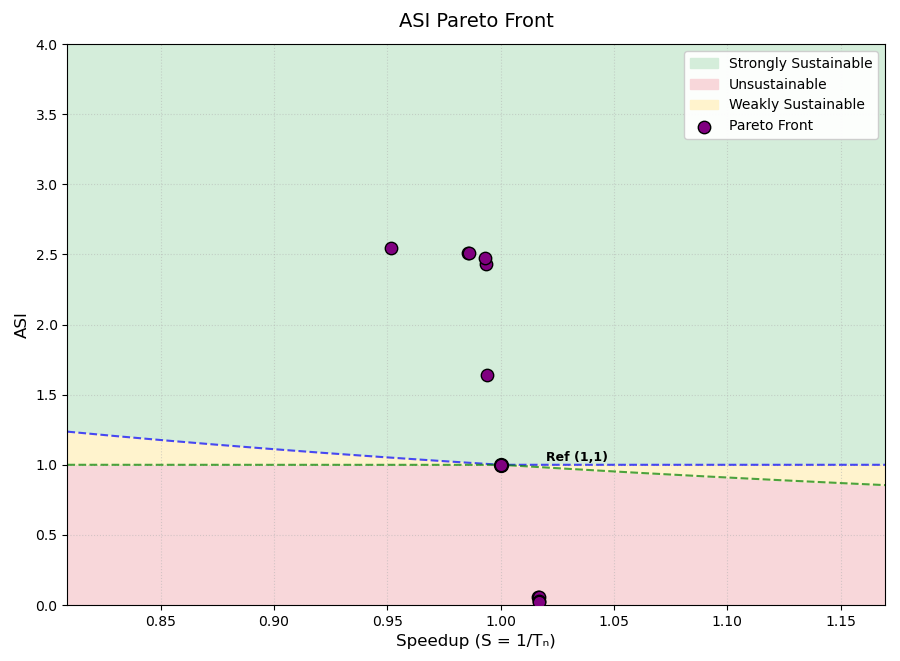
\includegraphics[width=0.48\textwidth]{../../images_results/ML2_CCl_MIP_EI_mesmo_400_7.png}
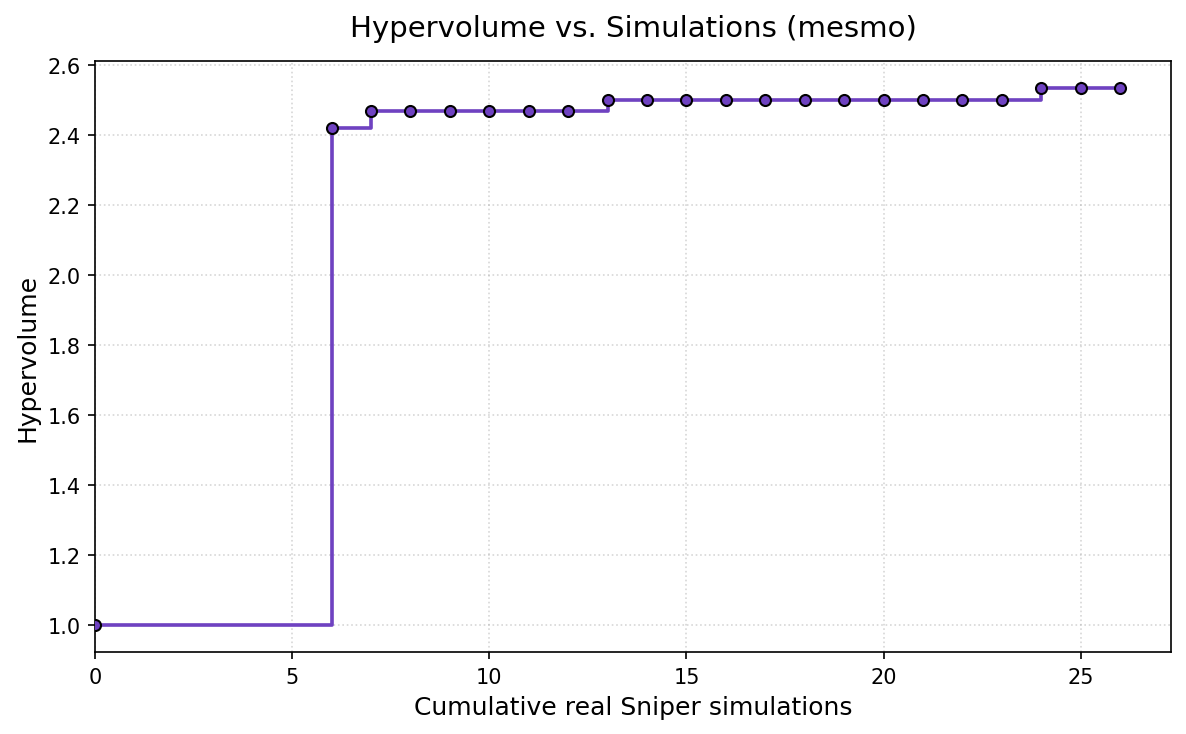
\includegraphics[width=0.48\textwidth]{../../images_results/ML2_CCl_MIP_EI_mesmo_400_7_hv_vs_sims.png}
\end{figure}

\textbf{Result:}
\newline
Total sniper runs: 26
\newline
Final hypervolume: 2.5351

\textbf{Front:}

\begin{table}[H]
\centering
\resizebox{\textwidth}{!}{%
\begin{tabular}{lllllllllllllllllllll}
\toprule
bpt & bp & l1da & l1d & l1ia & l1i & l2a & l2 & l3a & l3 & nhist & nnbl & nnlr & robc & robd & robw & ASI & Speedup & Area & PeakPow & Region \\
\midrule
a53 & 2048 & 8 & 32 & 8 & 32 & 4 & 512 & 8 & 2048 & 4 &  &  & 8 & 10 & 256 & 0.0244 & 1.0170 & 105.00 & 997.11 & Unsustainable \\
pentium\_m &  & 8 & 32 & 4 & 16 & 8 & 512 & 8 & 2048 &  &  &  & 8 & 8 & 512 & 0.0306 & 1.0169 & 108.38 & 762.95 & Unsustainable \\
a53 & 1024 & 8 & 64 & 8 & 16 & 8 & 512 & 8 & 1024 & 3 &  &  & 10 & 8 & 256 & 0.0583 & 1.0169 & 81.53 & 535.21 & Unsustainable \\
a53 & 1024 & 8 & 16 & 8 & 16 & 8 & 512 & 8 & 1024 & 3 &  &  & 10 & 8 & 256 & 0.0591 & 1.0163 & 80.08 & 535.08 & Unsustainable \\
baseline &  &  &  &  &  &  &  &  &  &  &  &  &  &  &  & 1.0000 & 1.0000 & 94.01 & 27.56 & Reference \\
pentium\_m &  & 4 & 64 & 8 & 16 & 4 & 256 & 4 & 2048 &  &  &  & 2 & 2 & 512 & 1.6414 & 0.9940 & 44.46 & 25.64 & Strongly Sust. \\
pentium\_m &  & 4 & 16 & 8 & 16 & 4 & 256 & 4 & 2048 &  &  &  & 2 & 2 & 256 & 2.4282 & 0.9933 & 42.61 & 17.56 & Strongly Sust. \\
pentium\_m &  & 4 & 16 & 8 & 16 & 4 & 256 & 4 & 2048 &  &  &  & 2 & 2 & 64 & 2.4777 & 0.9933 & 42.43 & 17.23 & Strongly Sust. \\
tage &  & 4 & 16 & 8 & 16 & 4 & 256 & 4 & 2048 &  &  &  & 2 & 2 & 32 & 2.5100 & 0.9862 & 42.37 & 17.01 & Strongly Sust. \\
pentium\_m &  & 4 & 16 & 8 & 16 & 4 & 256 & 4 & 2048 &  &  &  & 2 & 2 & 32 & 2.5104 & 0.9857 & 42.37 & 17.01 & Strongly Sust. \\
nn &  & 4 & 16 & 8 & 16 & 4 & 256 & 4 & 2048 &  & 64 & 0.001 & 2 & 2 & 32 & 2.5457 & 0.9516 & 42.37 & 16.77 & Strongly Sust. \\
\bottomrule
\end{tabular}
}
\end{table}


\item 100 iterations

\begin{figure}[H]
\centering
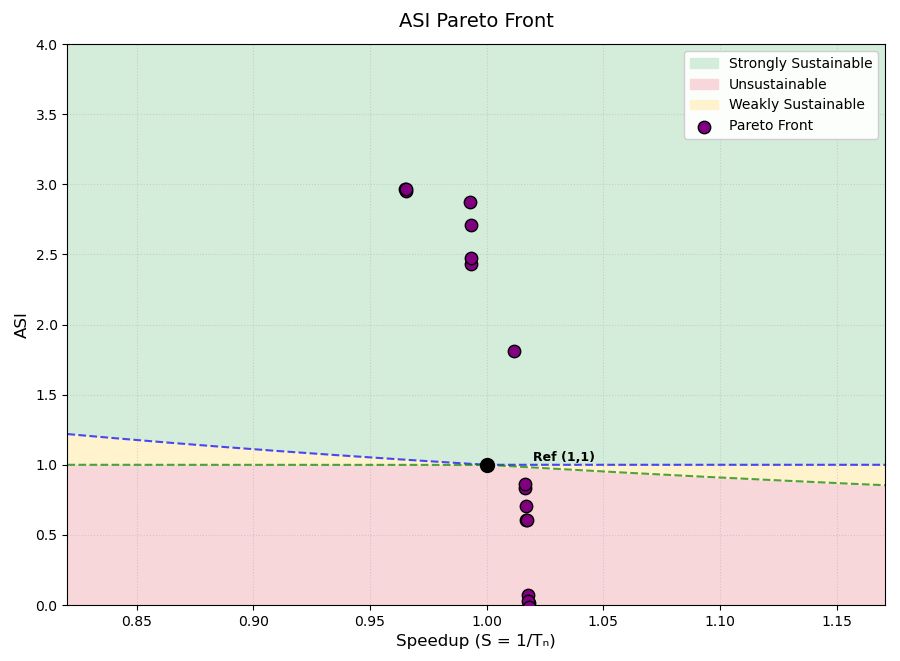
\includegraphics[width=0.48\textwidth]{../../images_results/ML2_CCl_MIP_EI_mesmo_400_7_100iters.png}
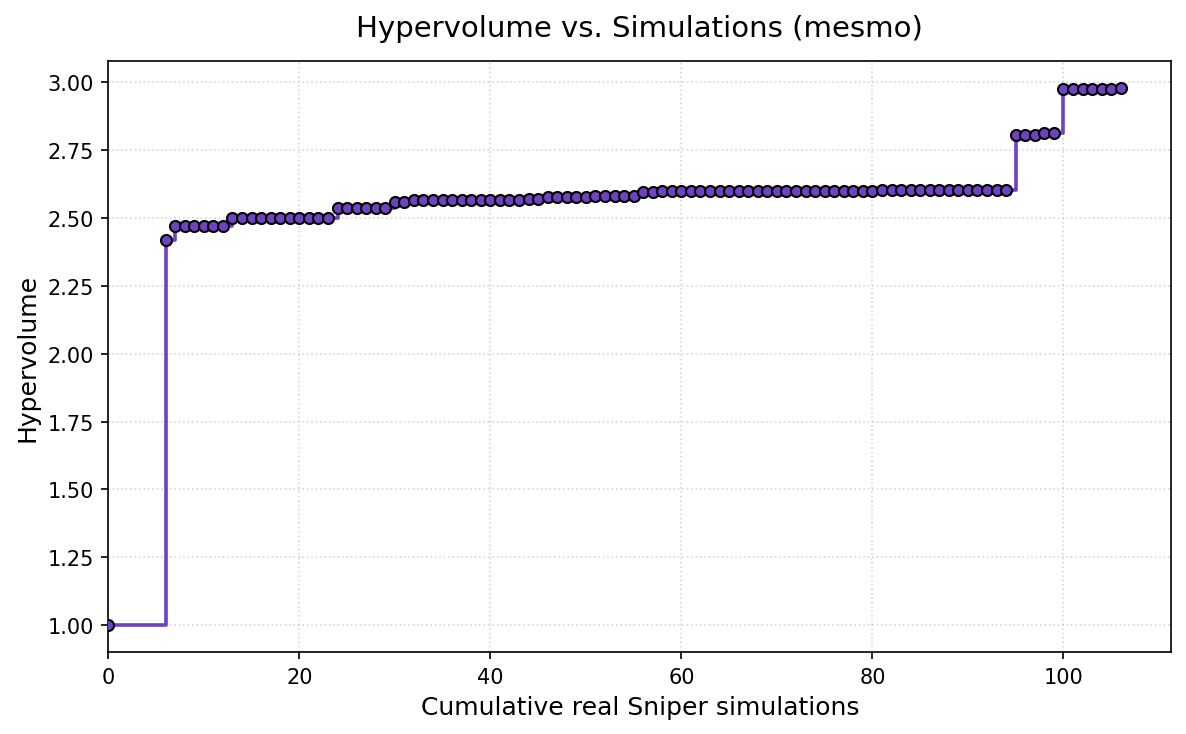
\includegraphics[width=0.48\textwidth]{../../images_results/ML2_CCl_MIP_EI_mesmo_400_7_100iters_hv_vs_sims.png}
\end{figure}

\textbf{Result:}
\newline
Total sniper runs: 106
\newline
Final hypervolume: 2.9794

\textbf{Front:}

\begin{table}[H]
\centering
\resizebox{\textwidth}{!}{%
\begin{tabular}{lllllllllllllllllllll}
\toprule
bpt & bp & l1da & l1d & l1ia & l1i & l2a & l2 & l3a & l3 & nhist & nnbl & nnlr & robc & robd & robw & ASI & Speedup & Area & PeakPow & Region \\
\midrule
tage &  & 4 & 64 & 8 & 16 & 4 & 512 & 16 & 8192 &  &  &  & 8 & 10 & 1024 & -0.0112 & 1.0180 & 288.40 & 2638.40 & Unsustainable \\
pentium\_m &  & 4 & 64 & 4 & 64 & 8 & 512 & 8 & 1024 &  &  &  & 10 & 10 & 512 & 0.0115 & 1.0180 & 131.82 & 1434.20 & Unsustainable \\
pentium\_m &  & 8 & 64 & 4 & 64 & 8 & 512 & 16 & 1024 &  &  &  & 8 & 10 & 256 & 0.0256 & 1.0177 & 101.17 & 995.75 & Unsustainable \\
pentium\_m &  & 8 & 64 & 4 & 64 & 8 & 512 & 16 & 1024 &  &  &  & 8 & 10 & 128 & 0.0690 & 1.0175 & 78.77 & 464.46 & Unsustainable \\
a53 & 2048 & 4 & 64 & 8 & 32 & 8 & 512 & 16 & 1024 & 4 &  &  & 8 & 10 & 64 & 0.6029 & 1.0171 & 63.08 & 60.76 & Unsustainable \\
pentium\_m &  & 8 & 32 & 4 & 16 & 8 & 512 & 4 & 1024 &  &  &  & 8 & 10 & 64 & 0.6048 & 1.0169 & 63.13 & 60.55 & Unsustainable \\
pentium\_m &  & 8 & 64 & 4 & 64 & 8 & 512 & 16 & 4096 &  &  &  & 8 & 8 & 64 & 0.7077 & 1.0167 & 77.22 & 45.90 & Unsustainable \\
a53 & 512 & 4 & 32 & 8 & 64 & 8 & 512 & 4 & 2048 & 4 &  &  & 10 & 8 & 64 & 0.8359 & 1.0163 & 62.05 & 44.18 & Unsustainable \\
a53 & 1024 & 4 & 32 & 4 & 32 & 4 & 512 & 16 & 2048 & 4 &  &  & 10 & 8 & 64 & 0.8658 & 1.0163 & 59.92 & 43.38 & Unsustainable \\
a53 & 512 & 8 & 32 & 4 & 16 & 8 & 512 & 8 & 1024 & 2 &  &  & 2 & 4 & 64 & 1.8109 & 1.0115 & 48.09 & 22.65 & Strongly Sust. \\
pentium\_m &  & 4 & 16 & 8 & 16 & 4 & 256 & 4 & 2048 &  &  &  & 2 & 2 & 256 & 2.4282 & 0.9933 & 42.61 & 17.56 & Strongly Sust. \\
pentium\_m &  & 4 & 16 & 8 & 16 & 4 & 256 & 4 & 2048 &  &  &  & 2 & 2 & 64 & 2.4777 & 0.9933 & 42.43 & 17.23 & Strongly Sust. \\
pentium\_m &  & 4 & 16 & 8 & 16 & 4 & 256 & 4 & 1024 &  &  &  & 2 & 2 & 64 & 2.7079 & 0.9931 & 35.48 & 16.52 & Strongly Sust. \\
a53 & 1024 & 4 & 32 & 4 & 16 & 4 & 256 & 4 & 1024 & 2 &  &  & 2 & 2 & 64 & 2.8713 & 0.9929 & 34.06 & 15.72 & Strongly Sust. \\
a53 & 512 & 4 & 64 & 4 & 16 & 4 & 256 & 4 & 1024 & 2 &  &  & 2 & 2 & 16 & 2.9494 & 0.9654 & 34.08 & 15.30 & Strongly Sust. \\
a53 & 1024 & 4 & 32 & 4 & 16 & 4 & 256 & 4 & 1024 & 2 &  &  & 2 & 2 & 16 & 2.9640 & 0.9653 & 33.91 & 15.24 & Strongly Sust. \\
a53 & 512 & 4 & 32 & 4 & 16 & 4 & 256 & 4 & 1024 & 2 &  &  & 2 & 2 & 16 & 2.9642 & 0.9651 & 33.91 & 15.24 & Strongly Sust. \\
\bottomrule
\end{tabular}
}
\end{table}
\end{itemize}
\subsection{SPEA2 - COLE}

\subsubsection{Hyperparameter settings 1}

Hyperparameter settings: Patience = 1 (amount of iterations to wait before stopping after no improvement), max\_iterations: int = 10. (max iter never reached)

\begin{figure}[H]
\centering
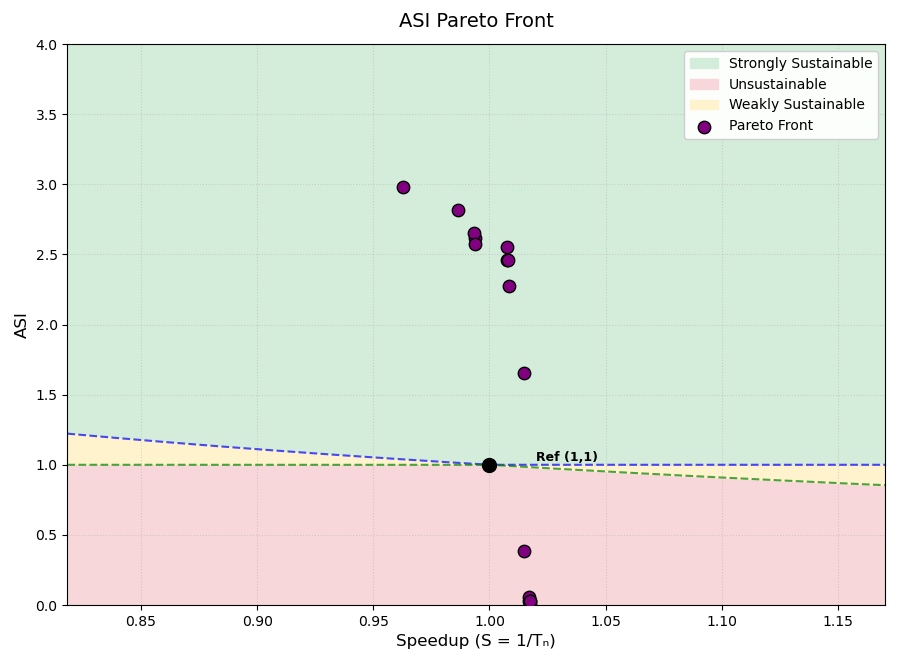
\includegraphics[width=0.48\textwidth]{../../images_results/ML2_CCl_MIP_EI_spea2.png}
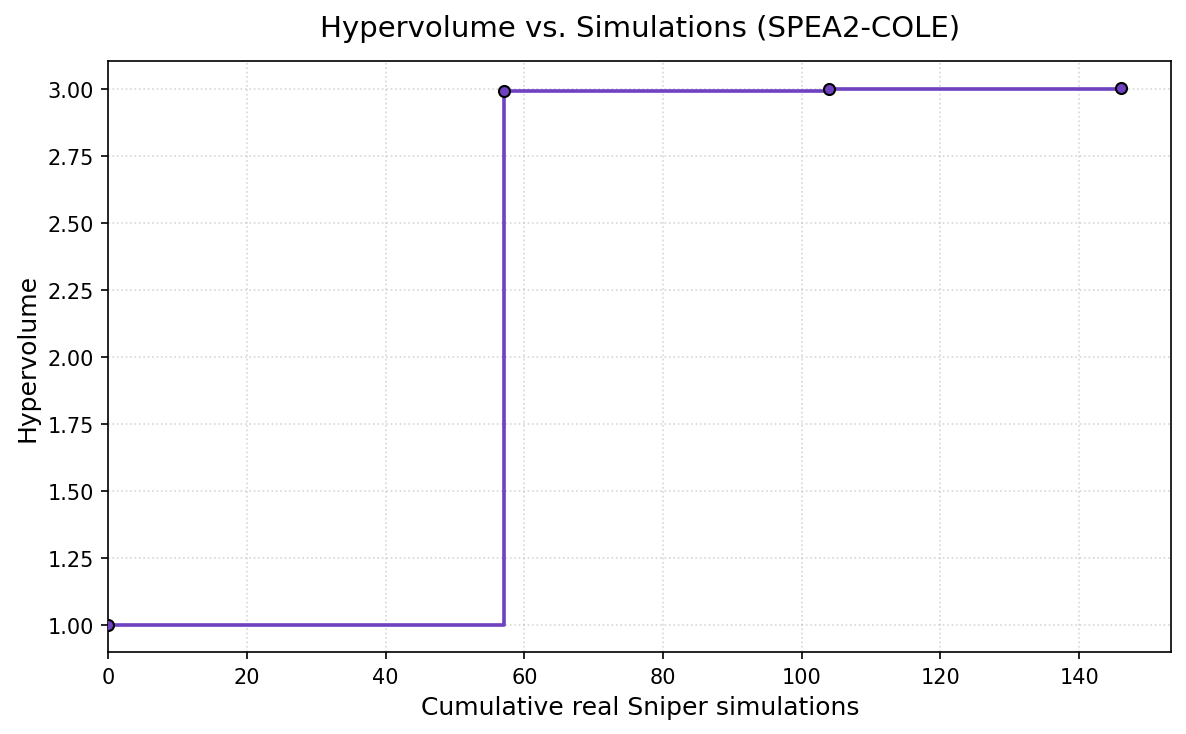
\includegraphics[width=0.48\textwidth]{../../images_results/ML2_CCl_MIP_EI_spea2_hv_vs_sims.png}
\end{figure}

\textbf{Result:}
\newline
Total sniper runs: 146
\newline
Final hypervolume: 3.0042

\textbf{Front:}

\begin{table}[H]
\centering
\resizebox{\textwidth}{!}{%
\begin{tabular}{lllllllllllllllllllll}
\toprule
bpt & bp & l1da & l1d & l1ia & l1i & l2a & l2 & l3a & l3 & nhist & nnbl & nnlr & robc & robd & robw & ASI & Speedup & Area & PeakPow & Region \\
\midrule
a53 & 2048 & 4 & 64 & 4 & 32 & 4 & 512 & 16 & 2048 & 3 &  &  & 8 & 10 & 512 & 0.0102 & 1.0176 & 138.09 & 1434.83 & Unsustainable \\
a53 & 2048 & 4 & 64 & 4 & 32 & 4 & 512 & 16 & 2048 & 3 &  &  & 8 & 10 & 256 & 0.0256 & 1.0174 & 100.93 & 995.54 & Unsustainable \\
pentium\_m &  & 4 & 32 & 4 & 32 & 8 & 512 & 16 & 2048 &  &  &  & 10 & 10 & 256 & 0.0257 & 1.0174 & 100.85 & 995.53 & Unsustainable \\
a53 & 1024 & 8 & 64 & 8 & 32 & 8 & 512 & 8 & 1024 & 3 &  &  & 4 & 8 & 512 & 0.0317 & 1.0171 & 105.48 & 763.17 & Unsustainable \\
tage &  & 4 & 32 & 8 & 32 & 4 & 512 & 16 & 4096 &  &  &  & 10 & 10 & 128 & 0.0603 & 1.0170 & 92.12 & 466.61 & Unsustainable \\
a53 & 1024 & 4 & 64 & 8 & 32 & 8 & 512 & 4 & 2048 & 3 &  &  & 8 & 4 & 512 & 0.3832 & 1.0150 & 60.14 & 97.85 & Unsustainable \\
tage &  & 8 & 64 & 4 & 32 & 4 & 512 & 8 & 2048 &  &  &  & 4 & 4 & 128 & 1.6527 & 1.0150 & 53.96 & 23.78 & Strongly Sust. \\
pentium\_m &  & 4 & 64 & 4 & 64 & 4 & 512 & 16 & 2048 &  &  &  & 8 & 2 & 256 & 2.2741 & 1.0084 & 48.86 & 17.94 & Strongly Sust. \\
pentium\_m &  & 4 & 64 & 4 & 32 & 8 & 512 & 16 & 1024 &  &  &  & 8 & 2 & 256 & 2.4611 & 1.0082 & 43.49 & 17.22 & Strongly Sust. \\
pentium\_m &  & 4 & 16 & 4 & 64 & 8 & 512 & 16 & 1024 &  &  &  & 2 & 2 & 256 & 2.4626 & 1.0077 & 43.71 & 17.18 & Strongly Sust. \\
a53 & 512 & 4 & 32 & 4 & 16 & 8 & 512 & 8 & 1024 & 3 &  &  & 4 & 2 & 128 & 2.5538 & 1.0074 & 40.89 & 16.89 & Strongly Sust. \\
pentium\_m &  & 8 & 32 & 4 & 64 & 4 & 256 & 4 & 1024 &  &  &  & 4 & 2 & 256 & 2.5740 & 0.9936 & 39.32 & 16.94 & Strongly Sust. \\
tage &  & 4 & 64 & 8 & 16 & 8 & 256 & 4 & 1024 &  &  &  & 8 & 2 & 256 & 2.6172 & 0.9936 & 36.56 & 16.97 & Strongly Sust. \\
pentium\_m &  & 4 & 16 & 8 & 16 & 4 & 256 & 4 & 1024 &  &  &  & 8 & 2 & 256 & 2.6515 & 0.9935 & 35.65 & 16.85 & Strongly Sust. \\
a53 & 512 & 4 & 32 & 4 & 32 & 4 & 128 & 16 & 1024 & 3 &  &  & 4 & 2 & 256 & 2.8159 & 0.9865 & 35.58 & 15.87 & Strongly Sust. \\
a53 & 512 & 4 & 16 & 4 & 32 & 8 & 128 & 16 & 1024 & 3 &  &  & 4 & 2 & 16 & 2.9808 & 0.9627 & 35.08 & 15.04 & Strongly Sust. \\
\bottomrule
\end{tabular}
}
\end{table}

\section{ML2 benchmark, larger working set}
Works with array where each element is 4 integers (32 bits) so 16 bytes. The size of the array used to be: 65536 * sizeof(el) = 65536 * 16 B = 1048576 B = 1 MiB
\newline
Pseudo random walk through this array.
\newline
Now we adjust the amount of elements to 65536 * 4 so we have 4 MiB
\newline
\newline
We expect each configuration where L3 is lower then working set to be really slow, and configuration with large enough L3 and maximum L2 size to be the fastest. (L3 size = 4 MiB already large enoug so I assume L3 size = 8 MiB will not be on front because larger ASI)
\newline
\newline
The Baseline (reference) has L2 size 256 and L3 size 8192 so I assume speedup can never be extremely large, in next simulation we will change baseline to L3 size to not fit the working set.
\newline
\newline
All folowing simulations are done with MESMO
\subsection{Reference: L3 size = 8 MiB, L2 size = 0.25 MiB}
\begin{figure}[H]
\centering
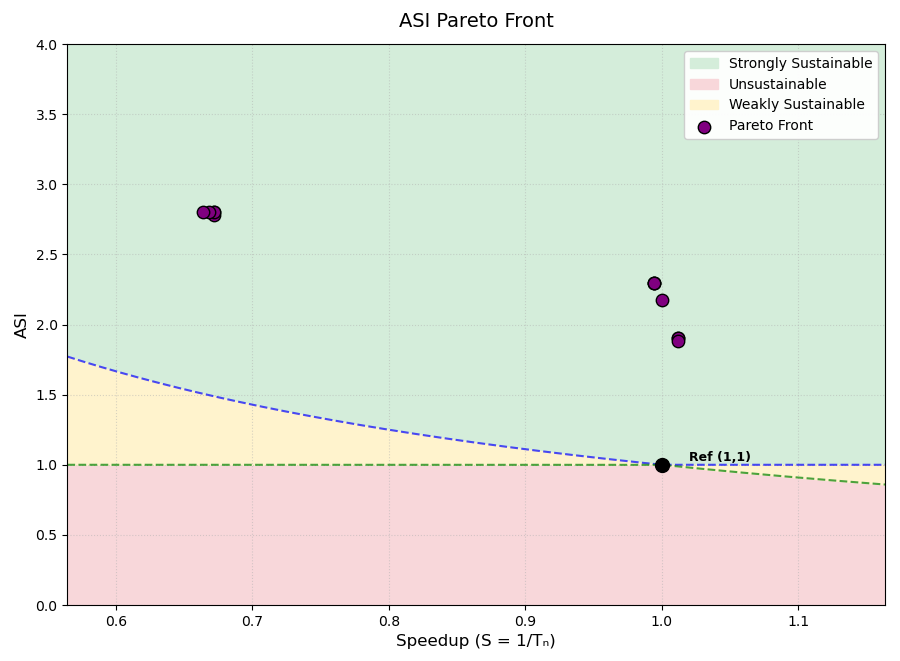
\includegraphics[width=0.48\textwidth]{../../images_results/ML2_4MiB_refL3_8MiB.png}
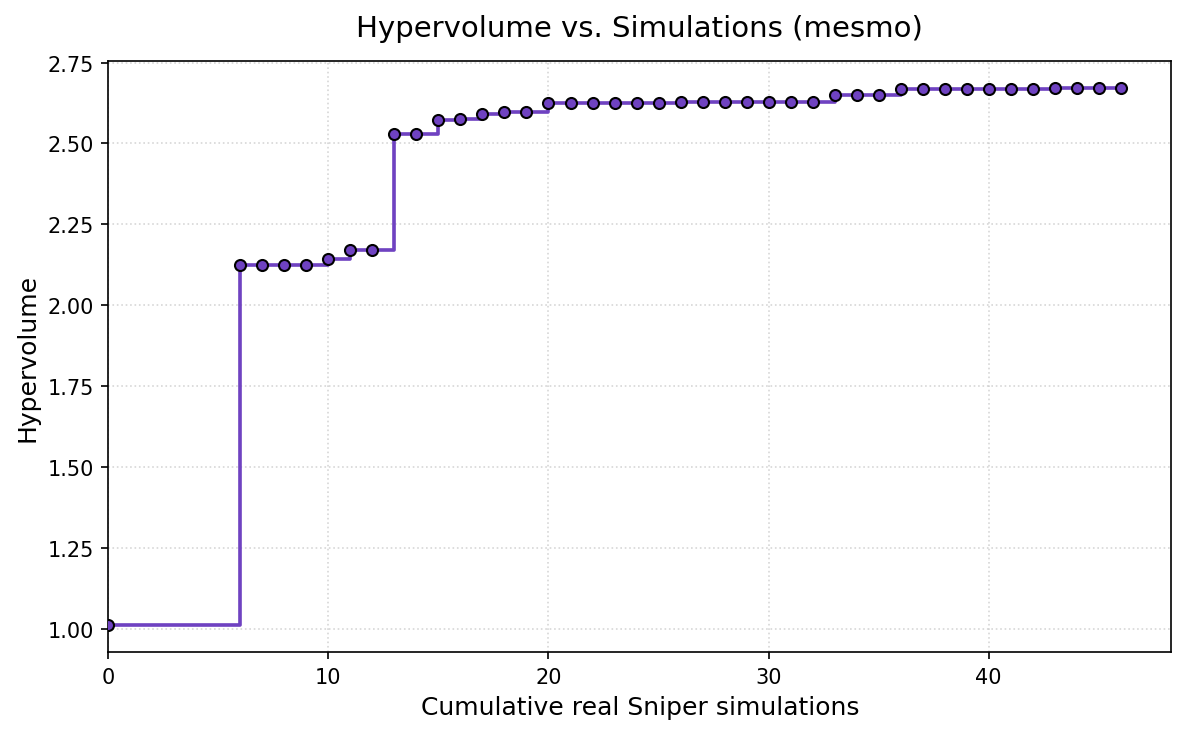
\includegraphics[width=0.48\textwidth]{../../images_results/ML2_4MiB_refL3_8MiB_hv_vs_sims.png}
\end{figure}

\textbf{Result:}
\newline
Total sniper runs: 46
\newline
Final hypervolume: 2.6719
\newline
I stopped after 40 iterations because we can see some points with L2 size to the maximum and L3 size 4 MiB have been found, aswell the complete opposite.
\newline
Right now I don't want to find complete front, I just want to see which clusters the search strategy can find.
\newline
\textbf{Front:}

\begin{table}[H]
\centering
\resizebox{\textwidth}{!}{%
\begin{tabular}{lllllllllllllllllllll}
\toprule
bpt & bp & l1da & l1d & l1ia & l1i & l2a & l2 & l3a & l3 & nhist & nnbl & nnlr & robc & robd & robw & ASI & Speedup & Area & PeakPow & Region \\
\midrule
pentium\_m &  & 8 & 64 & 4 & 16 & 4 & 512 & 4 & 4096 &  &  &  & 2 & 2 & 64 & 1.8803 & 1.0119 & 64.72 & 17.71 & Strongly Sust. \\
tage &  & 8 & 32 & 4 & 32 & 4 & 512 & 8 & 4096 &  &  &  & 8 & 2 & 32 & 1.9023 & 1.0117 & 64.54 & 17.53 & Strongly Sust. \\
a53 & 2048 & 8 & 32 & 4 & 32 & 4 & 512 & 8 & 4096 & 4 &  &  & 8 & 2 & 32 & 1.9023 & 1.0117 & 64.54 & 17.53 & Strongly Sust. \\
pentium\_m &  & 4 & 64 & 4 & 64 & 4 & 256 & 4 & 4096 &  &  &  & 4 & 2 & 128 & 2.1778 & 1.0002 & 54.51 & 16.55 & Strongly Sust. \\
a53 & 512 & 4 & 64 & 4 & 64 & 8 & 128 & 8 & 4096 & 4 &  &  & 2 & 2 & 16 & 2.2985 & 0.9944 & 53.33 & 15.82 & Strongly Sust. \\
nn &  & 4 & 64 & 4 & 64 & 8 & 128 & 8 & 4096 &  & 16 & 0.001 & 2 & 2 & 16 & 2.2985 & 0.9941 & 53.33 & 15.82 & Strongly Sust. \\
nn &  & 4 & 64 & 4 & 64 & 8 & 128 & 8 & 4096 &  & 64 & 0.005 & 2 & 2 & 16 & 2.2986 & 0.9940 & 53.33 & 15.82 & Strongly Sust. \\
pentium\_m &  & 4 & 64 & 8 & 64 & 4 & 256 & 8 & 2048 &  &  &  & 8 & 2 & 16 & 2.7839 & 0.6718 & 41.56 & 14.21 & Strongly Sust. \\
pentium\_m &  & 4 & 64 & 8 & 16 & 4 & 256 & 8 & 2048 &  &  &  & 2 & 2 & 16 & 2.8017 & 0.6718 & 40.90 & 14.18 & Strongly Sust. \\
tage &  & 4 & 64 & 8 & 16 & 4 & 256 & 8 & 2048 &  &  &  & 2 & 2 & 16 & 2.8017 & 0.6718 & 40.90 & 14.18 & Strongly Sust. \\
nn &  & 4 & 64 & 8 & 16 & 4 & 128 & 4 & 2048 &  & 64 & 0.0005 & 10 & 2 & 32 & 2.8026 & 0.6683 & 41.76 & 14.09 & Strongly Sust. \\
nn &  & 4 & 64 & 8 & 16 & 4 & 128 & 4 & 2048 &  & 64 & 0.0005 & 8 & 2 & 32 & 2.8046 & 0.6641 & 41.76 & 14.08 & Strongly Sust. \\
\bottomrule
\end{tabular}
}
\end{table}

\subsection{Reference: L3 size = 2 MiB, L2 size = 0.25 MiB}
We can not compare HV to other searches with other reference points, but we can look what kind of Front we get and which configurations are found.
\begin{figure}[H]
\centering
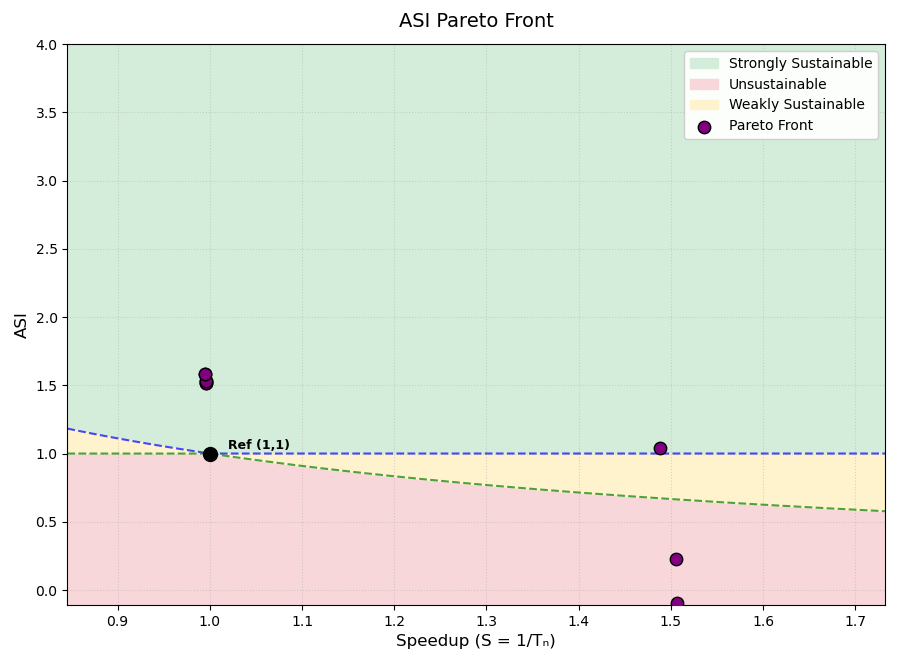
\includegraphics[width=0.48\textwidth]{../../images_results/ML2_4MiB_refL3_2MiB.png}
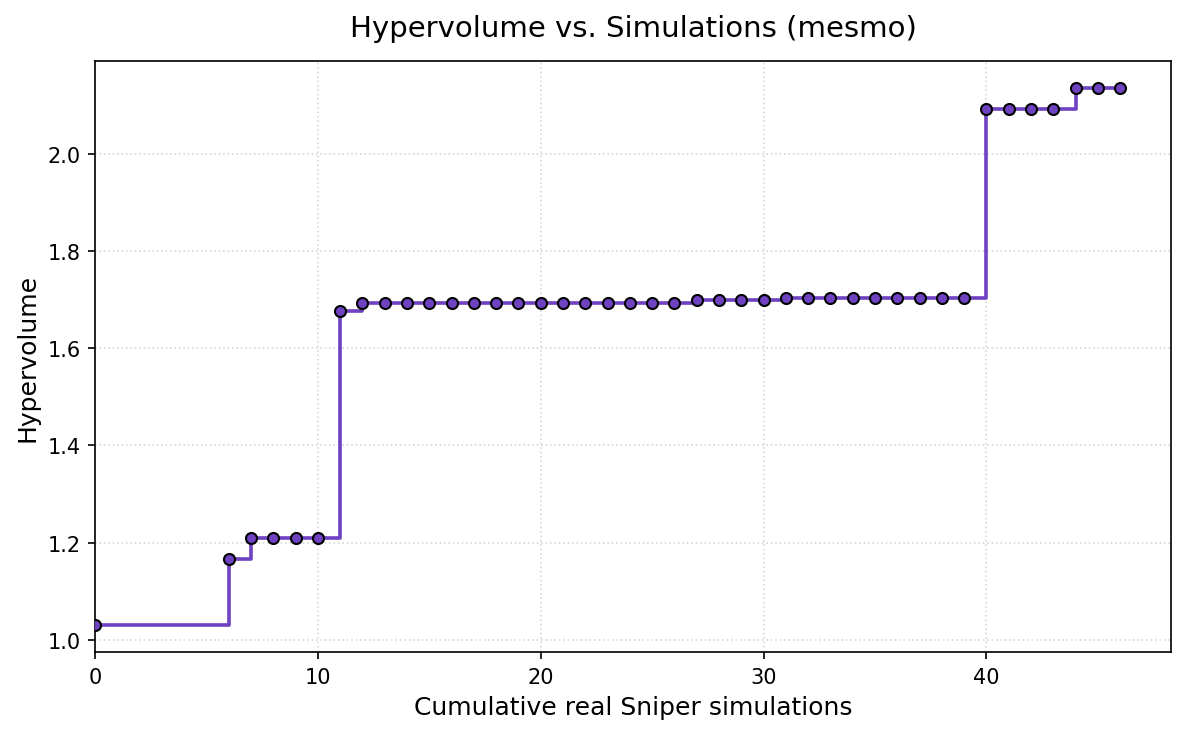
\includegraphics[width=0.48\textwidth]{../../images_results/ML2_4MiB_refL3_2MiB_hv_vs_sims.png}
\end{figure}

\textbf{Result:}
\newline
Total sniper runs: 46
\newline
Final hypervolume: 2.1357
\newline
\textbf{Front:}

\begin{table}[H]
\centering
\resizebox{\textwidth}{!}{%
\begin{tabular}{lllllllllllllllllllll}
\toprule
bpt & bp & l1da & l1d & l1ia & l1i & l2a & l2 & l3a & l3 & nhist & nnbl & nnlr & robc & robd & robw & ASI & Speedup & Area & PeakPow & Region \\
\midrule
a53 & 1024 & 8 & 32 & 8 & 16 & 8 & 512 & 8 & 8192 & 2 &  &  & 10 & 8 & 16 & -0.0957 & 1.5062 & 108.88 & 43.97 & Unsustainable \\
a53 & 1024 & 4 & 16 & 8 & 32 & 8 & 512 & 8 & 4096 & 2 &  &  & 10 & 8 & 64 & 0.2268 & 1.5059 & 73.96 & 43.61 & Unsustainable \\
pentium\_m &  & 4 & 16 & 8 & 64 & 8 & 256 & 4 & 4096 &  &  &  & 10 & 2 & 16 & 1.0418 & 1.4885 & 55.92 & 16.49 & Strongly Sust. \\
nn &  & 8 & 64 & 4 & 32 & 8 & 128 & 16 & 2048 &  & 64 & 0.001 & 4 & 2 & 64 & 1.5155 & 0.9962 & 44.89 & 14.27 & Strongly Sust. \\
a53 & 512 & 8 & 64 & 4 & 32 & 8 & 128 & 16 & 2048 & 4 &  &  & 4 & 2 & 64 & 1.5156 & 0.9961 & 44.89 & 14.27 & Strongly Sust. \\
a53 & 512 & 8 & 32 & 4 & 32 & 8 & 128 & 16 & 2048 & 3 &  &  & 4 & 2 & 64 & 1.5297 & 0.9960 & 44.55 & 14.23 & Strongly Sust. \\
nn &  & 8 & 32 & 4 & 32 & 8 & 128 & 16 & 2048 &  & 32 & 0.005 & 4 & 2 & 64 & 1.5297 & 0.9958 & 44.55 & 14.23 & Strongly Sust. \\
a53 & 512 & 8 & 32 & 4 & 32 & 8 & 128 & 4 & 2048 & 4 &  &  & 8 & 2 & 16 & 1.5796 & 0.9949 & 44.42 & 13.81 & Strongly Sust. \\
nn &  & 8 & 32 & 4 & 32 & 8 & 128 & 4 & 2048 &  & 32 & 0.005 & 8 & 2 & 16 & 1.5796 & 0.9948 & 44.42 & 13.81 & Strongly Sust. \\
\bottomrule
\end{tabular}
}
\end{table}

\section{Benchmarks}
\subsection{ML2}
ML2: L2 resident (depending on LFSR settings) linked list traversal.

\begin{lstlisting}[caption={ML2 benchmark source}]
#include <stdio.h>
#include <stdlib.h>     /* malloc, free, rand */

#include "common.h"

#define ASIZE 65536*4
#define STEP    128
#define ITERS  4096
#define LEN    2048


typedef struct dude {
  int p1,p2,p3,p4;
} dude;


dude arr[ASIZE];
__attribute__ ((noinline))
int loop(int zero) {
  int t = 0, count=0;

  unsigned lfsr = 0xACE1u;
  do
  {
      /* taps: 18 17 16 13; feedback polynomial: x^18 + x^17 + x^16 + x^13 + 1 */
      lfsr = (lfsr >> 1) ^ (-(lfsr & 1u) & 0x39000u);
      lfsr = lfsr + arr[lfsr].p1;
  //} while(++count < ITERS);
  } while(lfsr != 0xACE1u);

  return t;
}


int main(int argc, char* argv[]) {
   argc&=10000;
   ROI_BEGIN();
   int t=loop(argc);
   ROI_END();
   volatile int a = t;
}
\end{lstlisting}

\subsection{CCl}
CCl: Impossible control with large basic blocks (potentially larger penalty)

\begin{lstlisting}[caption={CCl benchmark source}]
    #include <stdio.h>
#include "randArr.h"
#include "common.h"

#define ASIZE 2048
#define STEP   256
#define ITERS    8

__attribute__ ((noinline))
int loop(int zero) {
  int t = 0,i,iter;
  for(iter=0; iter < ITERS; ++iter) {
    for(i=0; i < STEP + zero; i+=1) {
      if(randArr[i])  {
        t+=3+3*t;
        t&=0xFFF;
        t+=3+3*t;
        t&=0xFFF;
        t+=3+3*t;
        t&=0xFFF;
        t+=3+3*t;
        t&=0xFFF;
        t+=3+3*t;
        t&=0xFFF;
        t+=3+3*t;
        t&=0xFFF;
        t+=3+3*t;
        t&=0xFFF;
        t+=3+3*t;
        t&=0xFFF;
        t+=3+3*t;
        t&=0xFFF;
      } else {
        t&=0xFFF;
        t+=3+3*t;
        t&=0xFFF;
        t+=3+3*t;
        t&=0xFFF;
        t+=3+3*t;
        t&=0xFFF;
        t+=3+3*t;
        t&=0xFFF;
        t+=3+3*t;
        t&=0xFFF;
        t+=3+3*t;
        t&=0xFFF;
        t+=3+3*t;
        t&=0xFFF;
        t+=3+3*t;
        t&=0xFFF;
        t+=3+3*t;
      }
    }
  }
  return t;
}

int main(int argc, char* argv[]) {
   argc&=10000;
   ROI_BEGIN(); 
   int t=loop(argc); 
   ROI_END();
   volatile int a = t;
}

\end{lstlisting}

\subsection{MIP}
MIP: Large Instruction Region -- Instruction cache Misses

\begin{lstlisting}
    #include <stdio.h>
#include "common.h"

#define ASIZE 2048
#define STEP   128
#define ITERS    4

__attribute__ ((noinline))
int loop(int zero) {
  int t = zero,i,iter;
  for(iter=0; iter < ITERS; ++iter) {
    t += 1;
    t *= 2;
    t -= 1;
    t &= 0xFFF00FFF;
    t ^= 0x14022;
    t %= 0xFFFFFF3;
    t += 6;
    t *= 10;
    t += 1;
    t *= 2;
    t -= 1;
    t &= 0xFFF00FFF;
    t ^= 0x14022;
    t %= 0xFFFFFF3;
    t += 6;
    t *= 10;
    t += 1;
    t *= 2;
    t -= 1;
    t &= 0xFFF00FFF;
    t ^= 0x14022;
    t %= 0xFFFFFF3;
    ...
    t += 1;
    t *= 2;
    t -= 1;
    t &= 0xFFF00FFF;
    t ^= 0x14022;
    t %= 0xFFFFFF3;
    t += 6;
    t *= 10;
  }
  return t;
}

int main(int argc, char* argv[]) {
   argc&=10000;
   ROI_BEGIN(); 
   int t=loop(argc); 
   ROI_END();
   volatile int a = t;
}
\end{lstlisting}

\subsection{EI}
EI:Integer Execution -- 8 Independent computations per iteration 

\begin{lstlisting}
    #include <stdio.h>
#include "common.h"

#define ASIZE 2048
#define STEP   128
#define ITERS 4096

__attribute__ ((noinline))
int loop(int zero) {
  int t1 = 1;
  int t2 = 89;
  int t3 = 3;
  int t4 = 21;
  int t5 = 2;
  int t6 = 7;
  int t7 = 2;
  int t8 = 3;
  int t9 = 1;
  int t10 = 89;
  int t11 = 3;
  int t12 = 21;
  int t13 = 2;
  int t14 = 7;
  int t15 = 2;
  int t16 = 3;

  int i;

  for(i=zero; i < ITERS; i+=1) {
    t1+=i;
    t2+=i;
    t3+=i;
    t4+=i;
    t5+=i;
    t6+=i;
    t7+=i;
    t8+=i;
    t9+=i;
    t10+=i;
    t11+=i;
    t12+=i;
    t13+=i;
    t14+=i;
    t15+=i;
    t16+=i;
  }
  return t1+t2+t3+t4+t5+t6+t7+t8*t9+t10+t11+t12+t13+t14+t15+t16;
}

int main(int argc, char* argv[]) {
   argc&=10000;
   ROI_BEGIN(); 
   int t=loop(argc); 
   ROI_END();
   volatile int a = t;
}

\end{lstlisting}
\end{document}

